\documentclass[11pt,a4paper]{article}

% ---------------------------------------------------------------------------------------------
% Prototype quantum neural networks under realistic noise — reproduction, noise study,
% hardware plan and shot-noise programme.  Every number is traceable to a run directory under
% experiments/runs/ (gitignored) whose meta.json carries seed, git hash and backend; every figure
% is generated by experiments/report_figures.py from those run directories.
% Build: cd reports/tex && latexmk -pdf main.tex
% ---------------------------------------------------------------------------------------------

\usepackage[T1]{fontenc}
\usepackage[utf8]{inputenc}
\usepackage{lmodern}
\usepackage{microtype}
\usepackage[margin=2.4cm]{geometry}
\usepackage{amsmath,amssymb,amsthm}
\usepackage{graphicx}
\usepackage{booktabs}
\usepackage{array}
\usepackage{tabularx}
\usepackage{siunitx}
\usepackage{xcolor}
\usepackage{tikz}
\usepackage{quantikz}
\usepackage{caption}
\usepackage{subcaption}
\usepackage{enumitem}
\usepackage[section]{placeins}
\usepackage{url}
\usepackage{hyperref}
\usepackage[capitalise,nameinlink]{cleveref}

\hypersetup{colorlinks=true,linkcolor=blue!50!black,citecolor=blue!50!black,urlcolor=blue!50!black}
\captionsetup{font=small,labelfont=bf,width=0.95\textwidth}
\sisetup{detect-all,range-phrase=--,range-units=single}
\graphicspath{{figures/}}
\setlength{\parskip}{0.35em}

\providecommand{\ket}[1]{}\renewcommand{\ket}[1]{\lvert #1 \rangle}
\providecommand{\bra}[1]{}\renewcommand{\bra}[1]{\langle #1 \rvert}
\newcommand{\KL}{D_{\mathrm{KL}}}
\newcommand{\Pout}{P(\mathrm{out}=1)}
\newcommand{\RX}{R_X}
\newcommand{\CRX}{C\!R_X}
\newcommand{\TV}{\mathrm{TV}}
\newcommand{\code}[1]{\texttt{\small #1}}
\newcommand{\run}[1]{\texttt{\footnotesize #1}}
\newtheorem{definition}{Definition}

\title{Prototype quantum neural networks under realistic noise:\\
a reproduction, a calibrated noise study, a hardware plan,\\ and a shot-noise programme}
\author{Tobias J.~Osborne\thanks{Leibniz Universit\"at Hannover.  Code and run directories:
\texttt{prototype-learning} repository, sessions of 20--21 August 2026.}}
\date{21 August 2026}

\begin{document}
\maketitle

\begin{abstract}
We reproduce the four experiments of Rosenhahn and Hirche, \emph{Prototype Learning for Quantum
Neural Networks} \cite{ptqnn} --- a five-bit counting task, the Iris flowers, a Flappy Bird
controller and an ECG denoiser --- and then ask what happens to each of them on a real quantum
computer.  Three of the four reproduce (the fourth, the Iris weight picture of their Fig.~9,
does not); the numbers are in \cref{tab:scoreboard}.  We then build a noise layer from the
published calibration data of seven quantum computers (IBM, Quantinuum, IonQ, Google, IQM,
Rigetti), simulate every experiment under it exactly, and find that \emph{gate noise at today's
published levels does not break any of the small networks}: the bit-count histogram moves by a
total-variation distance of \numrange{0.005}{0.04}, the Flappy controller still plays perfectly
on all seven machines, and ECG denoising loses less than a decibel on the two machines we could
afford to simulate.  What does break them is the \emph{finite number of measurements}: the
Flappy controller's decisions sit a median of $0.019$ from its flap threshold, so it needs about
$10^4$ measurements per frame, and the bit-count loss is biased by $31.8/N$ at $N$
measurements.  We therefore develop and test three remedies --- margin-aware training,
common random numbers for the paper's finite-difference optimiser, and a sequential
measurement rule --- and find that the sequential rule alone cuts the Flappy measurement
budget by a factor of $4.6$ at no loss of play, that margin-aware training does not change the
margins that matter, and that common random numbers reduce the optimiser's derivative noise by
$3$--$30\times$ but cannot remove the bias of the plug-in loss.  A compilation and cost
study for each vendor closes with a concrete recommendation: run the seven-qubit Flappy
controller's activation map on a trapped-ion machine first.  Every number in this document is
produced by a script from a recorded run directory; every calibration figure carries a source
URL and a verbatim quotation; every choice the paper leaves open is marked as an assumption.
\end{abstract}

\tableofcontents

\section{Introduction}
\label{sec:intro}

\paragraph{What the paper proposes.}
A quantum neural network is a small quantum circuit whose rotation angles are treated as
trainable weights; the network's output is the probability of measuring one designated qubit in
the state $\ket{1}$.  Rosenhahn and Hirche \cite{ptqnn} propose a particular building block,
the \emph{prototype neuron}, in which each input qubit is first rotated by a learned angle, then
used to control a rotation of the neuron's own qubit, and finally rotated back
(\cref{fig:circuits}).  The effect is that the neuron ``fires'' most strongly when the input
pattern matches a stored prototype pattern, and the fact that the inputs are rotated back means
the same inputs can be shared by many neurons and by many training examples \emph{in
superposition}.  The paper demonstrates this on four tasks: learning a target histogram over all
32 five-bit strings at once (bit-count), classifying the Iris flowers, controlling a Flappy Bird
game, and denoising an electrocardiogram (ECG).  Training uses no gradient descent; it uses a
finite-difference estimate of the slope inside a simulated-annealing loop (\cref{sec:kwsa}).

\paragraph{What we did.}
This document records three things.  First, a \textbf{reproduction}: a clean-room implementation
(no code from the authors), cross-checked against an independent simulator written blind by a
second agent, that regenerates every figure and table of the paper that can be regenerated from
its text (\cref{sec:reproduction}).  Second, a \textbf{noise study}: a description of the seven
quantum computers for which vendors publish calibration data, as mathematical noise channels, and
an exact simulation of each experiment under each of them (\cref{sec:noise}), plus a
\textbf{compilation and cost study} of what it would take to run the circuits on each machine
(\cref{sec:hardware}).  Third, a \textbf{shot-noise programme}: having found that the number of
repeated measurements, not gate error, is what limits a hardware demonstration, we implement and
test three remedies (\cref{sec:shots}).

\paragraph{How to read the numbers.}
Every quantitative statement below comes from a \emph{run directory} --- a folder under
\code{experiments/runs/} holding the script's output together with the random seed, the commit
hash of the code and the simulator backend that produced it.  Run directories are named by
time stamp (for example \run{bitcount\_noise/20260820T145335Z}) and are quoted in the text; the
figures are produced from them by one script (\code{experiments/report\_figures.py}).  Where the
paper leaves a choice open (its optimiser step sizes, its train/test split, its game physics) we
had to choose, and each such choice is listed in \cref{app:assumptions}.  Every calibration
number of a quantum computer carries, in the repository, the URL it was read from, the date, and
a verbatim quotation (\cref{app:provenance}).

\paragraph{Compute discipline.}
Two machines were used.  Run directories from 25 September 2026 record the machine (host name,
platform, cores used) in their \code{meta.json}; for earlier ones the machine is attributed by
date.  The August 2026 runs --- the
reproduction, the noise study and the hardware plan, i.e.\ everything whose time stamp begins
\code{202608} --- ran on one workstation (64 cores, one RTX~3090 GPU).  Three runs of
18 September 2026 (\run{bitcount/20260918T111515Z}, \run{ecg/20260918T132924},
\run{iris/20260918T085641Z-drop}) ran on a 12-thread laptop with no GPU; the runs of
25 September (\code{20260925}) ran on the workstation again, from clean commits, and reproduce
to the last recorded digit every laptop number they overlap (the laptop run directories are not
on the workstation; the comparison is against the values recorded from them).  Wall times are quoted with the number of cores
actually used.  No single run was allowed to exceed about two
hours; two studies that would have (noise-aware training of the 11-qubit bit-count network,
$\approx 13$ hours for its grid; the full ECG/Iris noise grid, $\approx 8$ hours) were
deliberately \emph{not} run and are reported as such, with their measured per-cell cost, rather
than approximated.  The ECG reruns on the paper's own recording use the $1\,800$-sample
Fig.~13 window, with the full recording as a check (\cref{sec:ecg}).

\begin{table}[t]
\centering\small
\caption{Scoreboard: what the paper reports and what we obtain.  ``Reproduced'' means the
qualitative claim and the quantitative value (within the precision the paper's figure allows)
both come out; ``discrepancy'' means they do not, and the text explains what we tried.}
\label{tab:scoreboard}
\begin{tabularx}{\textwidth}{@{}>{\raggedright\arraybackslash}p{0.21\textwidth} >{\raggedright\arraybackslash}p{0.21\textwidth} X >{\raggedright\arraybackslash}p{0.16\textwidth}@{}}
\toprule
Paper item & Paper value & Ours & Status \\
\midrule
Fig.~3, activation surface & $(0,1)\!\to\!\max$, $(1,0)\!\to\!0$ & $1.000$ / $0.000$ / $0.500$ / $0.500$ at the corners & reproduced \\
Fig.~5, target histogram & bar heights & $(\text{number of ones}+1)/112$, all 32 bars within $0.0002$ & reproduced \\
Fig.~6, superposition training & $\KL\approx 0$ in $\approx 8$ iterations & median $<0.005$ at sweep 9; $5/6$ seeds $<10^{-3}$ at 20 & reproduced \\
Fig.~6, iterative baseline & $\KL\approx 0$ by $\approx 120$ & per-input $\KL<10^{-3}$ for $4/6$ seeds within $10^5$ elementary steps (a fifth reaches $1.4\times10^{-3}$); the superposition $\KL$ is a different observable & reproduced in the per-input observable; iteration unit assumed \\
Fig.~7, Iris learning curves & classic overfits, prototype does not & classic test loss rises after 1--4 sweeps; prototype's keeps falling; over 20 seeds the classic test loss ends $>5\,\%$ above its minimum on 8 (merge) / 7 (drop), the prototype's on 2 / 0 & reproduced \\
Iris accuracy & $\approx 98\,\%$ & $95$ / $91$ / $98\,\%$ on three splits (ceilings $97$ / $99$ / $99\,\%$); over 20 seeds $94.3\pm2.8\,\%$ (classic $93.9\pm2.7\,\%$), $96.4\,\%$ on the filtered set when ambiguous codes are dropped & $2$--$4$ points short; no architecture advantage \\
Fig.~9, Iris weight picture & prototype weights span the data & t-SNE: both weight sets cluster away from the data.  Scored over 20 seeds: the prototype layer covers more codes than the classic one, but already does so untrained; training makes it more selective, yet less so than the classic layer; angles do not decode to data patterns & discrepancy (criterion fixed in advance) \\
Flappy Bird & ``plays perfectly'' & $110/110$ pipes (the cap) on $20/20$ held-out games & reproduced (own clone) \\
Table~I, ECG PSNR (1/2/3 hidden) & $32.9$ / $40.00$ / $40.04$~dB & $37.4$ / $38.0$ / $38.1$~dB (synthetic signal); $36.8$ / $37.5$ / $36.9$~dB on the paper's own recording ($37.8$ / $37.8$ / $36.2$~dB on all $7\,700$ samples) & within $\approx 2$~dB on synthetic; on the original recording 1-neuron reproduced, 2/3-neuron $2$--$4$~dB short \\
\bottomrule
\end{tabularx}
\end{table}

\section{Notation and definitions}
\label{sec:notation}

This section defines every symbol used later.  A reader who knows quantum circuits can skim it;
a reader who does not should find here everything needed to follow the rest.

\paragraph{Qubits, states, measurement.}
A \emph{qubit} is a two-level quantum system with basis states $\ket{0}$ and $\ket{1}$.  The
state of $n$ qubits is a unit vector $\psi \in \mathbb{C}^{2^n}$ whose components are indexed by
$n$-bit strings; we write the string with \emph{qubit~1 (the first input) as the most significant
bit}, matching the paper's circuit figures, which number qubits from the top.  Measuring all
qubits returns the bit string $x$ with probability $|\psi_x|^2$.  When only some qubits are
measured, the probability of their outcome is the sum of $|\psi_x|^2$ over the strings $x$ that
agree with it on those qubits (the \emph{marginal}).  A \emph{mixed} state, needed as soon as
noise enters, is a positive matrix $\rho$ of unit trace (the \emph{density matrix}); a pure state
is $\rho=\psi\psi^\dagger$, and measurement probabilities are its diagonal entries.

\paragraph{Gates.}
A gate is a unitary matrix acting on one or two qubits.  The ones the paper uses are
\begin{align}
\RX(\theta) &= \begin{pmatrix}\cos\frac{\theta}{2} & -i\sin\frac{\theta}{2}\\[2pt]
-i\sin\frac{\theta}{2} & \cos\frac{\theta}{2}\end{pmatrix}, \qquad
H = \tfrac{1}{\sqrt2}\begin{pmatrix}1&1\\1&-1\end{pmatrix}, \\
\CRX(\theta) &= \ket{0}\bra{0}\otimes I + \ket{1}\bra{1}\otimes \RX(\theta)
\quad\text{(rotate the target by $\theta$ only if the control is $\ket{1}$).}
\end{align}
$\RX(\theta)\ket{0} = \cos\frac{\theta}{2}\ket{0} - i\sin\frac{\theta}{2}\ket{1}$, so after
$\RX(\theta)$ a qubit prepared in $\ket{0}$ is measured as $1$ with probability
$\sin^2(\theta/2)$.  $H$ turns $\ket{0}$ into the equal superposition
$(\ket{0}+\ket{1})/\sqrt2$; $H$ on every input qubit prepares all $2^n$ input strings at once with
equal weight.

\paragraph{Encoding a real number as an angle.}
A feature value $s\in[0,1]$ enters the circuit as $\RX(\theta(s))$ on its input qubit.  The paper
does not state $\theta(s)$; its companion paper \cite{snn} (Fig.~4) prints
$\CRX(1.369)$ for the value $0.4$ and $\CRX(1.7722)$ for $0.6$, which pins
\begin{equation}
\theta(s) = 2\arcsin\sqrt{s}, \qquad\text{so that } P(\text{qubit reads } 1) = s .
\label{eq:encoding}
\end{equation}
We use \cref{eq:encoding} throughout and report the alternative $\theta = \pi s$ as an ablation
where it matters (ECG, \cref{sec:ecg}).

\paragraph{Networks and their output.}
A network has $n_{\mathrm{in}}$ input qubits, $n_{\mathrm{hid}}$ hidden qubits (one per hidden
neuron) and one output qubit; $n = n_{\mathrm{in}}+n_{\mathrm{hid}}+1$.  Its output for a given
input is the \emph{activation}
\begin{equation}
\Pout \;=\; \Pr[\text{output qubit reads }1],
\end{equation}
a number in $[0,1]$.  For a classifier it is thresholded (Flappy: flap iff $\Pout>\tfrac12$);
for a regressor it is the predicted value (ECG: the denoised sample).

\paragraph{The superposition observable and the training loss.}
For the bit-count and Iris tasks the inputs are prepared in superposition and the measured joint
distribution of (input string $x$, output bit) is read.  The \emph{model distribution} is
\begin{equation}
q(x) \;=\; \frac{P(\text{inputs}=x,\ \mathrm{out}=1)}{\sum_{x'} P(\text{inputs}=x',\ \mathrm{out}=1)},
\label{eq:model-distribution}
\end{equation}
i.e.\ the input distribution \emph{conditioned on the output having fired} --- the output
amplitude acts as a weight on each input pattern (paper, Fig.~4 caption).  It is compared to a
target distribution $p(x)$ by the Kullback--Leibler divergence (paper, Eq.~(4)),
\begin{equation}
\KL(p\,\|\,q) \;=\; \sum_x p(x)\,\log\frac{p(x)}{q(x)} \;\ge 0,
\qquad \KL = 0 \iff p = q,
\label{eq:kl}
\end{equation}
with $0\log 0 = 0$ and $q$ floored at $10^{-12}$ so the value stays finite (our choice; the paper
does not say).  A second dissimilarity we use for noise is the \emph{total-variation distance}
$\TV(p,q) = \tfrac12\sum_x |p(x)-q(x)| \in [0,1]$, the largest difference in probability that any
event can have under the two distributions.

\paragraph{Noise channels.}
Real gates are not unitary.  A \emph{channel} is a linear map $\rho\mapsto\sum_i K_i\rho K_i^\dagger$
with $\sum_i K_i^\dagger K_i = I$ (the $K_i$ are its \emph{Kraus operators}); it sends density
matrices to density matrices.  Three channels describe a calibrated machine:
\begin{itemize}[nosep]
\item \emph{Depolarising} with probability $p$: with probability $1-p$ nothing happens, with
probability $p$ the state of the affected qubit(s) is replaced by the maximally mixed state.  A
vendor's ``average gate error'' $\varepsilon$ is converted to $p$ by
$\varepsilon = p\,(1 - 2^{-k})\,\tfrac{2^k}{2^k+1}$ for a $k$-qubit gate ($p = 2\varepsilon$ for
one qubit, $p = \tfrac{4}{3}\cdot\tfrac{5}{4}\varepsilon$ for two), which makes the channel's
average fidelity equal to $1-\varepsilon$ (cross-checked against Qiskit~Aer).
\item \emph{Relaxation} over a time $t$ with the vendor's $T_1$ (energy decay time) and $T_2$
(phase decay time): $\ket{1}$ decays toward $\ket{0}$ with probability $1-e^{-t/T_1}$ and
superpositions lose coherence by $e^{-t/T_2}$.  It is applied during every gate (for its
duration) and during every idle interval, which we schedule as early as possible, exactly as
IBM's compiler does.
\item \emph{Readout confusion}: the recorded bit differs from the true one with probability
$p_{01}$ (true $0$ read as $1$) or $p_{10}$ (true $1$ read as $0$).
\end{itemize}
The resulting \emph{noise model} of a machine is the rule ``after each gate, apply the gate's
depolarising channel and its relaxation; on every idle qubit, apply relaxation for the idle time;
at the end, apply readout confusion''.  Its parameters come from the vendor data of
\cref{app:provenance}; a \emph{noise scale} $s$ multiplies all of $p$, $1/T_1$, $1/T_2$ and the
readout errors together ($s=1$ is the published machine, $s=0$ is noiseless).

\paragraph{Shots.}
A quantum computer does not return probabilities; it returns one bit string per run, and
probabilities are estimated by repeating the circuit $N$ times (\emph{$N$ shots}).  An estimate
$\hat p = k/N$ of a probability $p$ has standard deviation $\sqrt{p(1-p)/N}\le 1/(2\sqrt N)$.  We
call $\delta = |\Pout - \tfrac12|$ the \emph{decision margin} of a thresholded output: a frame
decided from $N$ shots is decided wrongly with probability $\approx\Phi(-2\delta\sqrt N)$, where
$\Phi$ is the standard normal distribution function.

\paragraph{Fidelity.}
For a compiled circuit on a given machine we quote the estimate
\begin{equation}
F \;\approx\; \prod_{\text{2q gates}}(1-\varepsilon_{2})\;\prod_{\text{1q gates}}(1-\varepsilon_{1})\;
\prod_{\text{qubits}} F_{\mathrm{idle}}(t)\;\prod_{\text{qubits}}\bigl(1-\tfrac{p_{01}+p_{10}}{2}\bigr),
\label{eq:fidelity}
\end{equation}
the probability that no error at all occurred in the run, with
$F_{\mathrm{idle}}(t) = \tfrac12 + \tfrac16\bigl(2e^{-t/T_2}+e^{-t/T_1}\bigr)$ the average
fidelity of relaxation over the circuit's duration $t$ \cite{nielsen}.  It is a first-order
bookkeeping estimate, not a simulation; the simulations are reported next to it.

\paragraph{Abbreviations.}
KW--SA: the paper's optimiser (\cref{sec:kwsa}).  PSNR: peak signal-to-noise ratio,
$10\log_{10}(R^2/\mathrm{MSE})$ with $R$ the signal range and MSE the mean squared error, in
decibels (dB).  SSIM: structural similarity index \cite{wang}, a number in $[0,1]$ comparing
local means, variances and covariance of two signals.  SWAP: the gate that exchanges two qubits,
inserted by a compiler when a two-qubit gate is requested between qubits that are not physically
connected; it costs three native two-qubit gates.

\section{The models and the optimiser}
\label{sec:models}

\subsection{Classic and prototype neurons}
\label{sec:neurons}

\begin{figure}[t]
\centering
\begin{subfigure}[b]{0.36\textwidth}\centering
\resizebox{\linewidth}{!}{\begin{quantikz}[row sep=0.35cm, column sep=0.45cm]
\lstick{$q_1$ (input)} & \ctrl{2} & \qw & \qw \\
\lstick{$q_2$ (input)} & \qw & \ctrl{1} & \qw \\
\lstick{$q_3$ (neuron)} & \gate{\RX(w_1)} & \gate{\RX(w_2)} & \gate{\RX(b)} \qw
\end{quantikz}}
\caption{Classic neuron (paper, Fig.~1): one controlled rotation per input and a bias
rotation on the neuron's qubit.  The inputs are untouched.}
\end{subfigure}\hfill
\begin{subfigure}[b]{0.6\textwidth}\centering
\resizebox{\linewidth}{!}{\begin{quantikz}[row sep=0.35cm, column sep=0.4cm]
\lstick{$q_1$} & \gate{\RX(\varphi_1)} & \ctrl{2} & \gate{\RX(-\varphi_1)} & \qw & \qw & \qw \\
\lstick{$q_2$} & \qw & \qw & \qw & \gate{\RX(\varphi_2)} & \ctrl{1} & \gate{\RX(-\varphi_2)} \\
\lstick{$q_3$} & \qw & \gate{\RX(\theta)} & \qw & \qw & \gate{\RX(\theta)} & \qw
\end{quantikz}}
\caption{Prototype neuron (paper, Fig.~2): each input is rotated by a learned $\varphi_i$,
controls a rotation by the \emph{same} $\theta$ of the neuron's qubit, and is rotated back.}
\end{subfigure}
\caption{The two neuron types.  A network (paper, Figs.~4, 5, 10, 12) is a layer of
$n_{\mathrm{hid}}$ hidden neurons, each touching all $n_{\mathrm{in}}$ inputs, followed by one
classic output neuron controlled by the hidden qubits.  Our implementation
(\code{ptqnn.circuits.neurons}) builds exactly these gate lists; the un-computation
$\RX(-\varphi_i)$ is what lets several prototype neurons share the same inputs and what lets a
dataset be presented in superposition.}
\label{fig:circuits}
\end{figure}

\Cref{fig:circuits} shows the two neuron types as circuits.  The \emph{classic} neuron is the
quantum perceptron of \cite{snn}: its qubit receives a bias rotation $\RX(b)$ and one controlled
rotation $\CRX(w_i)$ from each input; the inputs are left unchanged.  The \emph{prototype}
neuron rotates input $i$ by $\RX(\varphi_i)$, lets it control a rotation by a shared angle
$\theta$ of the neuron qubit, and rotates it back by $\RX(-\varphi_i)$.  The pair
$(\varphi_1,\dots,\varphi_{n_{\mathrm{in}}})$ is the stored \emph{prototype}: when the input
state is the one that $\RX(-\varphi_i)$ would map to $\ket{1}$ on every qubit, every controlled
rotation fires and the neuron's activation is maximal; when no input matches, none fires and the
activation is zero (\cref{fig:activation}).  A network uses prototype (or, for comparison,
classic) hidden neurons and always a classic output neuron.  Parameter counts: the 11-qubit
bit-count network (5 inputs, 5 hidden) has $5\times(5+1) + (5+1) = 36$ angles; the 7-qubit Flappy
network (2 inputs, 4 hidden) has $4\times 3 + 5 = 17$.

A sanity check that a reader can verify by hand: a single prototype neuron with two inputs,
prototype $(\pi, 0)$ and $\theta = \pi/2$, fed the basis input $(0,1)$, gives $\Pout = 1$; fed
$(1,0)$ it gives $0$; fed $(0,0)$ or $(1,1)$ it gives $\tfrac12$.  \Cref{fig:activation} is this
neuron's activation over all real-valued inputs --- the paper's Fig.~3.  The paper's own surface
bottoms out near $0.2$ rather than $0$, because its parameters (not given) differ from these.

\begin{figure}[t]
\centering
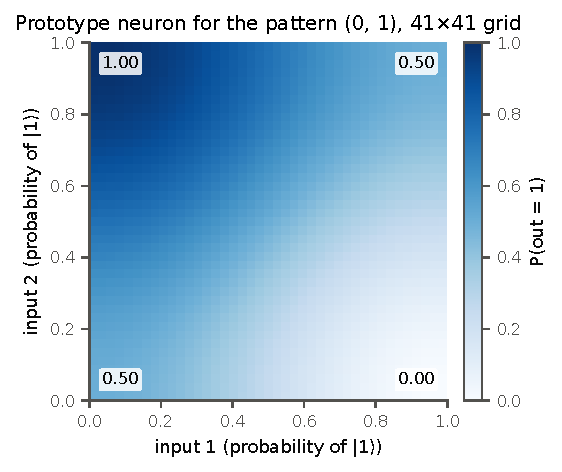
\includegraphics[width=0.46\textwidth]{fig_activation_surface}
\caption{Activation $\Pout$ of one prototype neuron with prototype $(0,1)$ as a function of
the two inputs (each given as the probability that its qubit reads $1$, encoded by
\cref{eq:encoding}).  The corner values are exact.  Run \run{bitcount/20260820T135930Z}.}
\label{fig:activation}
\end{figure}

\subsection{The optimiser: finite differences inside simulated annealing}
\label{sec:kwsa}

The paper trains with no gradient descent.  It estimates the slope of the loss $f$ along one
parameter by the \emph{central difference} $\bigl(f(x+c\,e_i) - f(x-c\,e_i)\bigr)/2c$
(Kiefer--Wolfowitz \cite{kw}), proposes a step against it, and accepts or rejects the proposal by
the \emph{Metropolis rule} of simulated annealing: always accept a decrease of the loss, accept
an increase $\Delta$ with probability $e^{-\Delta/kT}$ at temperature $T$ (paper, Eq.~(3)),
cooling $T$ geometrically.  Neither paper gives the step sizes $a_n$ and $c_n$, the
temperature schedule or what one ``iteration'' is, so the following is our choice (listed in
\cref{app:assumptions}): $a_n = a_0/(n+1)^{0.602}$, $c_n = c_0/(n+1)^{0.101}$ (Spall's standard
exponents \cite{spall}); one \emph{sweep} visits every parameter once in random order, evaluates
the two probes $x\pm c_n e_i$ and the proposed step, and puts the best of the three to the
Metropolis rule.  One sweep therefore costs $3\times(\text{number of parameters})$ circuit
evaluations --- $108$ for the bit-count network.  Whole-vector steps (one gradient estimate of all
parameters, then one step) stalled near $\KL\approx 10^{-2}$ at every setting tried, so the
coordinate sweep is the default; it is what \cref{fig:convergence} shows.  For a rotating
mini-batch of training episodes (Flappy) the incumbent loss is re-evaluated every sweep, because
comparing a candidate scored on one batch against an incumbent scored on another is meaningless
(\cref{sec:flappy}).

\subsection{Simulators}
\label{sec:simulators}

The reference simulator is plain NumPy (state vectors for noiseless runs, density matrices for
noisy ones) and is the oracle for everything else: an independent density-matrix simulator
written blind by a second agent agrees with it to $10^{-12}$ on random circuits; a C density-matrix
library (\code{orkan}), a Monte-Carlo trajectory simulator for circuits too large for density
matrices (Iris at 17 qubits), a GPU density-matrix backend, and one shared batched state-vector
kernel used by all task-specific fast paths are each tested against it on \emph{full output
distributions}, never only on $\Pout$.  The noise model's idle scheduling reproduces Qiskit's
as-soon-as-possible scheduler delay for delay, and its channels agree with Qiskit~Aer's on a
noisy three-qubit circuit to $2\times 10^{-15}$.

\section{Reproduction of the four experiments}
\label{sec:reproduction}

\subsection{Bit-count: learning a histogram over all inputs at once}
\label{sec:bitcount}

\paragraph{Task.}
Five input qubits are placed in equal superposition of all 32 strings; the network is trained so
that the model distribution \cref{eq:model-distribution} matches a target histogram that rises
with the number of ones in the string.  The paper gives the target only as a bar chart
(Fig.~5, bottom right); reading the bars gives $p(x) = (\text{number of ones in } x + 1)/112$
for every one of the 32 bars to within $0.0002$ ($112 = \sum_x (\text{ones}+1)$ is the
normalisation).  The network is the paper's Fig.~5: 5 inputs, 5 prototype hidden neurons, one
classic output, 11 qubits.

\paragraph{Result.}
\Cref{fig:histograms} shows the target and the trained model: $\KL = 5.5\times10^{-4}$.  (The
paper's own printed model histogram, read off the figure, has $\KL\approx 2.6\times10^{-3}$
against the same target.)  \Cref{fig:convergence} (left) is the paper's Fig.~6: from a random
start the median of six optimiser seeds crosses $\KL = 0.005$ at sweep~9 and five of six seeds
are below $10^{-3}$ at sweep~20; one seed stalls at $0.014$.  The paper reports ``$\approx 0$ in
about 8 iterations'' without defining an iteration; against our sweeps it matches.

\paragraph{The iterative baseline does not reproduce.}
The paper's Fig.~6 also shows a slower ``iterative'' curve, training on one input at a time and
reaching $\approx 0$ by about 120 iterations.  The paper describes this only as ``optimizing
examples iteratively''; the companion paper \cite{snn} describes sample-wise squared-error updates
with the same optimiser but gives no schedule.  Our construction --- one optimiser sweep on the
squared error of one randomly chosen input per iteration --- stalls at a median $\KL\approx 0.15$
after 200 iterations (\cref{fig:convergence}, right), and a sweep over step sizes $a_0\in\{2,5,20,
50,100\}$, two decay exponents, both update modes and a scaled per-sample target left the median
between $0.05$ and $0.3$ (best single run $0.046$).  Updating on one input at a time thrashes
between inputs.  We record this as a discrepancy: whatever the authors' iterative scheme was, ours
is not it.

\begin{figure}[t]
\centering
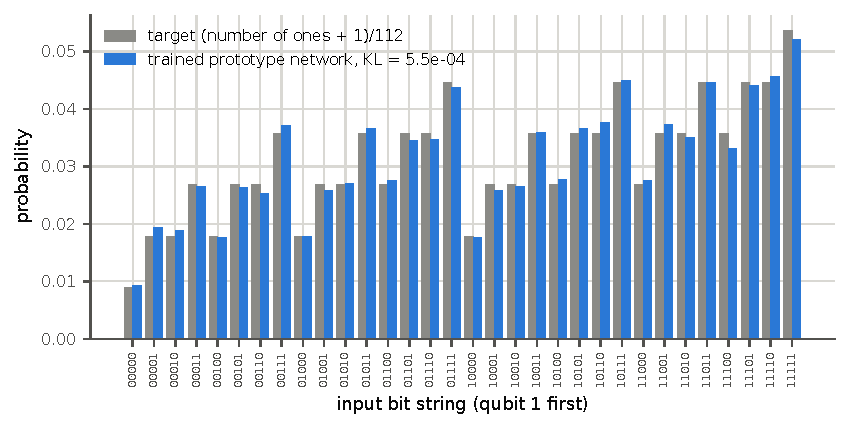
\includegraphics[width=\textwidth]{fig_bitcount_histograms}
\caption{Paper Fig.~5.  Target histogram (grey) and the trained prototype network's model
distribution (blue) over the 32 input strings.  Run \run{bitcount\_noise/20260820T145335Z}
(seed 1 of the bit-count training).}
\label{fig:histograms}
\end{figure}

\begin{figure}[t]
\centering
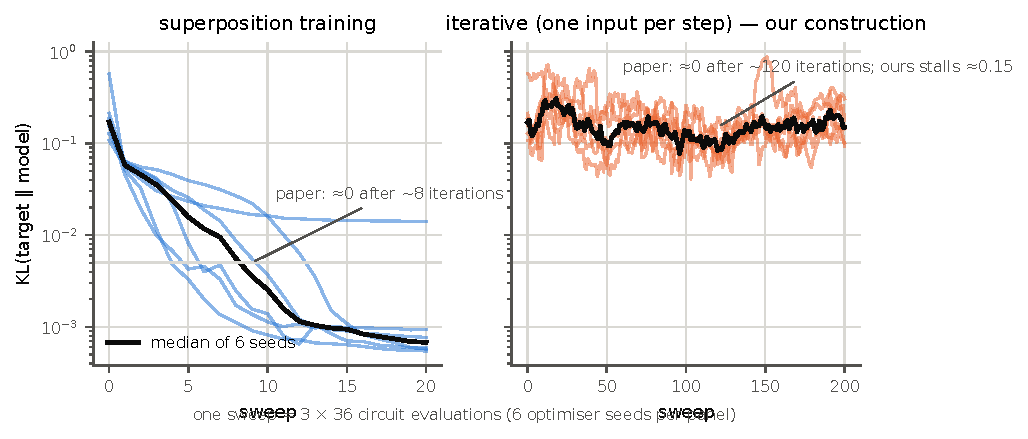
\includegraphics[width=\textwidth]{fig_bitcount_convergence}
\caption{Paper Fig.~6.  Left: superposition training, six seeds and their median.  Right:
our construction of the iterative baseline, which does not reach the paper's curve.  Run
\run{bitcount/20260820T135930Z}.}
\label{fig:convergence}
\end{figure}

\subsection{Iris: a dataset in superposition}
\label{sec:iris}

\paragraph{Task and encoding.}
Each of the four Iris features is quantised into three clusters by $k$-means, giving a 12-bit
one-hot code per flower; the whole training set is loaded as one superposition state over its
distinct codes, and the label is encoded in the amplitude.  The paper does not state how the
label enters; reading its Fig.~8 bar heights ($1/86, 4/86, 9/86$ on the training set and
$1/154, 4/154, 9/154$ on the test set, two independent integer normalisations) fixes the target
weight of class $\ell\in\{0,1,2\}$ to be proportional to $(\ell+1)^2$ --- the amplitude carries
$\ell+1$ and the histogram its square.  No other exponent produces both normalisations.  The
paper also does not state the train/test split; we use a stratified one-third training split
(50 flowers) and report the sensitivity.  The network has 12 inputs, 4 hidden neurons and one
output (17 qubits); a classic-neuron network of the same size is trained for comparison.
Predictions are made by reading each code's weight and rounding to the nearest label.

\paragraph{Result.}
\Cref{fig:iris-losses} is the paper's Fig.~7 on three data splits: the classic network drives
its training loss to $10^{-5}$ within a few sweeps while its test loss bottoms out early and
stays at $0.03$--$0.04$ (it memorises); the prototype network descends more slowly on both and
its test loss is still falling at sweep~40.  Test accuracy: $95\,\%$, $91\,\%$ and $98\,\%$ on
the three splits for the prototype network against a paper value of ``$\approx 98\,\%$''; the
encoding itself caps accuracy at $97\,\%$, $99\,\%$ and $99\,\%$ on those splits, because two
flowers of different species can share a 12-bit code.  \Cref{fig:iris-hist} is Fig.~8 for the
test split.  The Fig.~9 picture --- a two-dimensional embedding in which the prototype weights
are claimed to ``span the data'' --- does not reproduce: both weight sets cluster away from the
data in our embedding; we do not know what the authors plotted.

\paragraph{On the split.}
Fig.~8 shows 15 non-empty bars for the training set and 30 for the test set.  Our 50-flower
training splits produce 14, 12 and 14 distinct codes (close to 15), but the 100-flower test
splits produce only 20, 20 and 18 (not 30): a one-hot code with three clusters per feature does
not spread 100 flowers over 30 codes on any split we tried.  The figure therefore supports the
\emph{direction} of the split (test larger than train) but not its ratio, and the ratio remains
our assumption.

\begin{figure}[t]
\centering
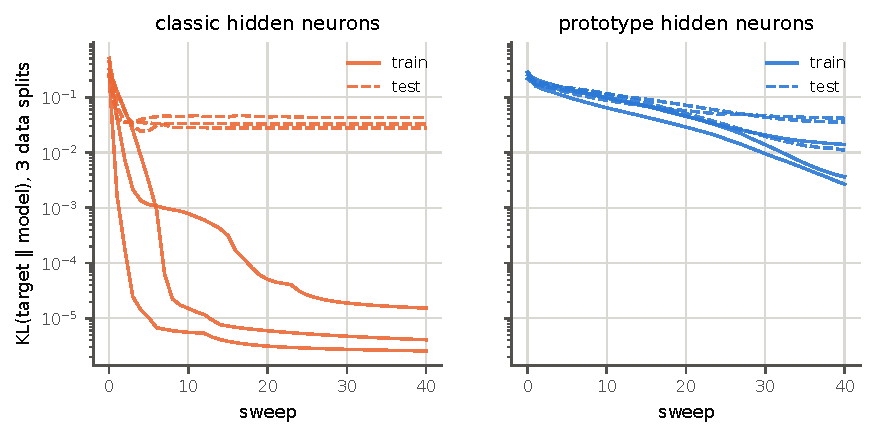
\includegraphics[width=\textwidth]{fig_iris_losses}
\caption{Paper Fig.~7.  Training (solid) and test (dashed) loss per sweep for three data splits.
Runs \run{iris/20260820T144849Z}, \run{…T145454Z}, \run{…T145455Z}.}
\label{fig:iris-losses}
\end{figure}

\begin{figure}[t]
\centering
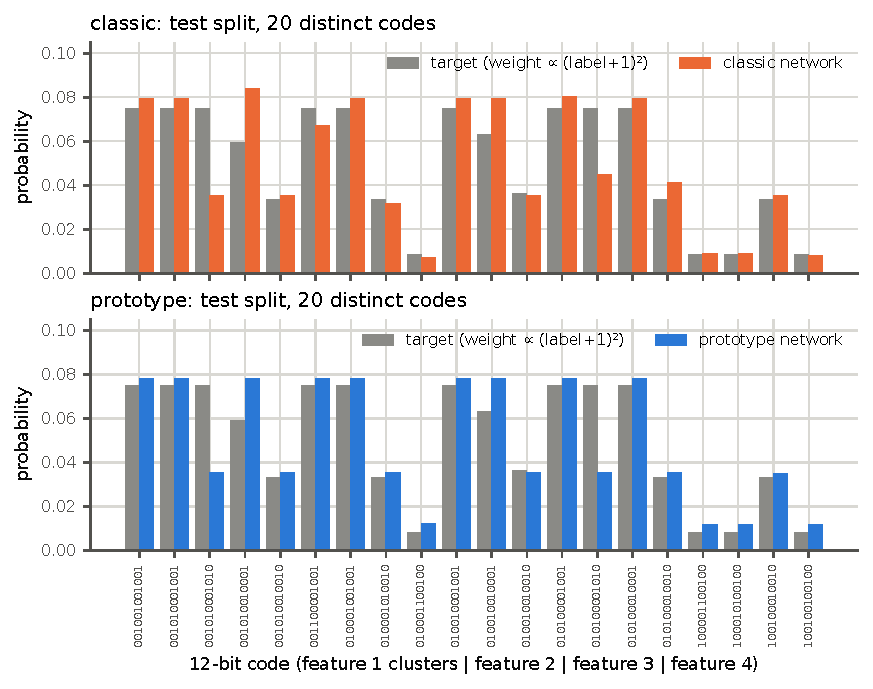
\includegraphics[width=\textwidth]{fig_iris_histograms}
\caption{Paper Fig.~8, test split of seed~0: target weight per distinct code (grey) against
the trained network's weight, classic (top) and prototype (bottom).  The bars are the
probabilities of reading each code together with the output firing, renormalised.}
\label{fig:iris-hist}
\end{figure}

\subsection{Flappy Bird: a seven-qubit controller}
\label{sec:flappy}

\paragraph{Task.}
Two features --- the bird's height and the centre of the next gap, both scaled to $[0,1]$ ---
enter two input qubits by \cref{eq:encoding}; four prototype hidden neurons and one classic
output decide ``flap'' when $\Pout > \tfrac12$ (paper, Fig.~10).  The paper says the trained
network ``plays the game perfectly'' and that a run was stopped after a score of 450\,000 that
took six days; it gives no reward, no training protocol and no game constants.  We built a
deterministic, window-free clone of the game.  Its physics are our choice: the classic
constants (flap impulse $-9$, gap 100, pipe spacing 144) are provably unplayable by a memoryless
policy on two features (one flap overshoots by 40.5 px against a 38 px budget), so we use impulse
$-7$, gap 120, spacing 180.  Training minimises the negative episode return (0.01 per frame
survived plus 1 per pipe) plus a small tracking term $|{\rm height} - {\rm gap}|$ that gives the
optimiser a slope in the region where every policy dies within 30 frames.  300 random parameter
vectors are scored on short episodes, the best seeds 25 sweeps of the optimiser on five
1500-frame training episodes.

\paragraph{Result.}
The trained network passes $110$ pipes in $5\,000$ frames --- the cap, i.e.\ a perfect game ---
on all 20 held-out game seeds, for all 8 optimiser seeds tried, in about three minutes of
training (run \run{flappy/20260820T143753Z}).  \Cref{fig:flappy-policy} shows what it learned: a
curved decision boundary in the (height, gap) plane, flapping when the bird is below the gap.  A
finding about the optimiser: rotating the five training episodes among a pool of ten every sweep
gave $0/25$ perfect games in the first session, and was recorded as a negative result; the cause
was that the optimiser kept its incumbent's loss from the previous batch, so every Metropolis
comparison compared scores on different games.  Re-scoring the incumbent on each new batch
restores $25/25$ perfect games (runs \run{flappy/batch0}, \run{flappy/batch5}), so the rotation
neither hurts nor helps here.

\begin{figure}[t]
\centering
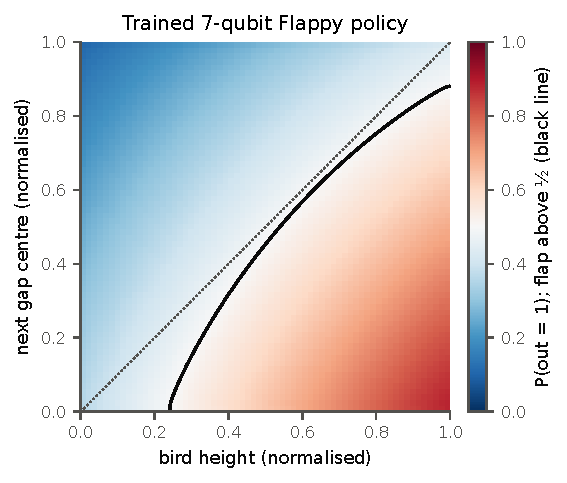
\includegraphics[width=0.5\textwidth]{fig_flappy_policy}
\caption{The trained Flappy controller's activation $\Pout$ over the two observations; the
black line is the decision boundary $\Pout = \tfrac12$ (flap to its right), the dotted diagonal
is ``bird at gap height''.  Run \run{flappy/20260820T143753Z}.}
\label{fig:flappy-policy}
\end{figure}

\subsection{ECG denoising}
\label{sec:ecg}

\paragraph{Task.}
A window of five consecutive noisy samples $s(t-2),\dots,s(t+2)$ enters five input qubits; one
to three prototype hidden neurons and one output predict the clean centre sample as $\Pout$
(paper, Fig.~12).  The paper does not say which recording it used; its Fig.~13 shows a smooth
two-beat trace of 1\,800 samples in $[0,1]$ with additive noise of standard deviation
$\approx 0.03$.  We generate a synthetic ECG of the McSharry form \cite{mcsharry} tuned to that
figure, add Gaussian noise of $\sigma = 0.02$ (noisy input $32.0$~dB), train on the first half and
test on the second, and repeat on PhysioNet MIT-BIH record~100 for comparison.  Quality is
measured by PSNR and SSIM (paper, Eqs.~(6)--(8)).

\paragraph{Result.}
\Cref{fig:ecg-trace} is the paper's Fig.~13; \cref{fig:ecg-table} is its Table~I.  We obtain
$37.4$, $38.0$ and $38.1$~dB for one, two and three prototype neurons against the paper's $32.9$,
$40.00$ and $40.04$: within about $2$~dB at two and three neurons, and $4$~dB \emph{above} the
paper at one neuron.  The prototype network beats the classic one at one and two neurons and on
every SSIM; the classic one wins at three.  Two notes.  The numbers cannot match exactly because
the signal is not the paper's; and the alternative angle encoding $\theta = \pi s$ costs
$0.6$--$7$~dB on this task, which is independent evidence for \cref{eq:encoding}.  On MIT-BIH
record~100 (run \run{ecg/20260820T165912}) the same networks reach $36$--$38$~dB.

\begin{figure}[t]
\centering
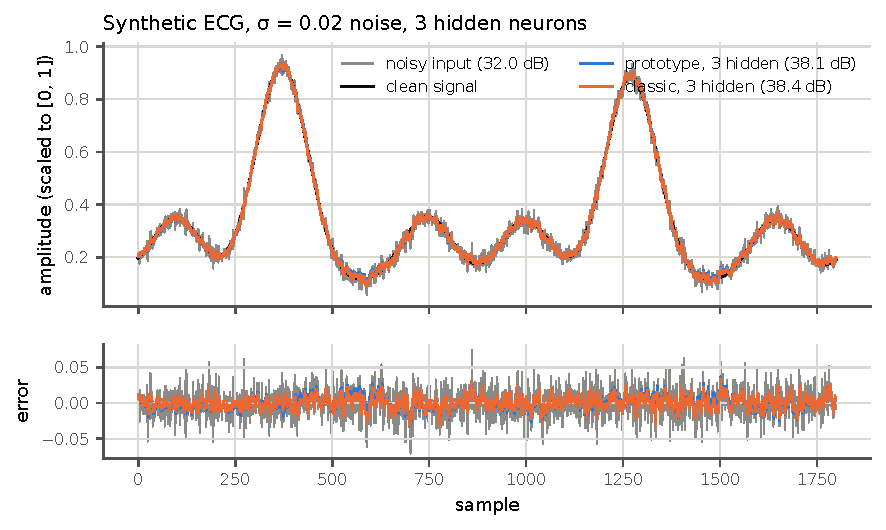
\includegraphics[width=\textwidth]{fig_ecg_trace}
\caption{Paper Fig.~13.  Noisy input, clean signal and the two three-neuron networks' outputs
(top); their errors (bottom).  Run \run{ecg/20260820T162014}.}
\label{fig:ecg-trace}
\end{figure}

\begin{figure}[t]
\centering
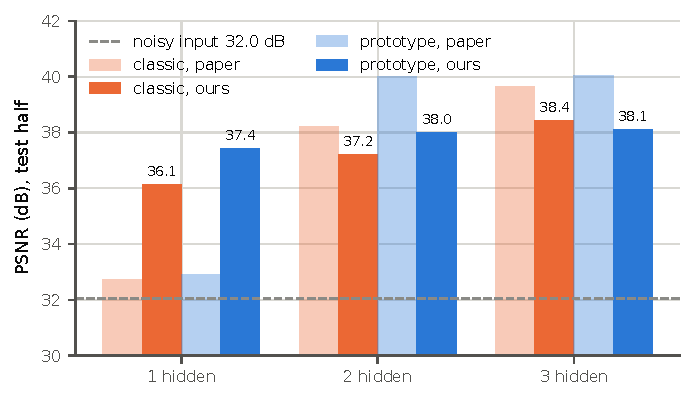
\includegraphics[width=0.7\textwidth]{fig_ecg_table}
\caption{Paper Table~I as a chart: PSNR on the test half for one to three hidden neurons,
paper values (light) against ours (dark).  Run \run{ecg/20260820T162014}.}
\label{fig:ecg-table}
\end{figure}

\section{The experiments under calibrated noise}
\label{sec:noise}

\subsection{Seven machines as noise models}
\label{sec:devices}

For each of seven quantum computers we collected the vendor's published calibration numbers
--- two-qubit and one-qubit gate error, gate durations, $T_1$, $T_2$, readout error, and the
qubit connectivity --- into a device file whose every field carries the URL it was read from,
the retrieval date (20 August 2026) and a verbatim quotation (\cref{app:provenance}).
\Cref{tab:devices} summarises them.  Three things are worth knowing before reading any noise
result.  \emph{Quantinuum publishes no gate durations and no $T_1$/$T_2$}; its idle error is
instead charged from its published ``memory error per depth-1 circuit time''
($2.0\times10^{-4}$ for H2-1, $2.2\times10^{-4}$ for H1-1), and its simulated noise contains
no idle error at all.  \emph{Rigetti publishes only a two-qubit error} for Ankaa-3 (and the
99.5\,\% headline is for a different gate than the universal one we need); every Rigetti number
below is therefore an upper bound on the machine.  \emph{IQM's $T_1$/$T_2$ are a third-party
snapshot}, not vendor data, and its $T_2$ measured without echo is $8.5$\,µs against the
$21$\,µs echo value we use.  Where a vendor publishes no number we model that channel as
error-free and say so, rather than invent one.

\begin{table}[t]
\centering\small
\caption{The seven device presets (medians where the vendor publishes per-qubit tables).
Two-qubit error $\varepsilon_2$, one-qubit error $\varepsilon_1$, readout error (mean of
$p_{01}$, $p_{10}$), coherence times, two-qubit gate time.  ``—'' = not published; the
provenance of every entry is in \cref{app:provenance}.}
\label{tab:devices}
\begin{tabular}{@{}l l S[table-format=1.2e-1] S[table-format=1.1e-1] S[table-format=1.1e-1] l l S[table-format=5.0]@{}}
\toprule
Machine & Connectivity & {$\varepsilon_2$} & {$\varepsilon_1$} & {readout} & $T_1$ & $T_2$ & {2q gate (ns)} \\
\midrule
Quantinuum H1-1 & all-to-all & 9.7e-4 & 1.8e-5 & 2.3e-3 & — & — & {—} \\
Quantinuum H2-1 & all-to-all & 1.1e-3 & 1.9e-5 & 1.0e-3 & — & — & {—} \\
IonQ Forte & all-to-all & 4.0e-3 & 2.0e-4 & 5.0e-3 & 55\,s & 1\,s & 950000 \\
Google Willow & square & 4.1e-3 & 5.3e-4 & 8.0e-3 & 68\,µs & 89\,µs & 42 \\
IBM Fez (Heron r2) & heavy-hex & 3.9e-3 & 2.3e-4 & 7.7e-3 & 145\,µs & 88\,µs & 84 \\
IQM Garnet & square & 4.9e-3 & 8.0e-4 & 3.0e-2 & 27\,µs & 21\,µs & 30 \\
Rigetti Ankaa-3 & square & 1.0e-2 & {—} & {—} & — & — & 72 \\
\bottomrule
\end{tabular}
\end{table}

\subsection{Bit-count}
\label{sec:noise-bitcount}

The trained 11-qubit bit-count networks (prototype and classic) were evaluated exactly, as
density matrices on the GPU, under each preset
(run \run{bitcount\_noise/20260820T145335Z}; \cref{fig:bitcount-noise-devices}).  The model
distribution moves by a total-variation distance of $0.005$ (Quantinuum H2-1) to $0.039$ (IQM
Garnet); the KL to the target rises from $5.5\times10^{-4}$ to $7\times10^{-4}$ on H2-1 and to
$6\times10^{-3}$ on Garnet.  The prototype network is better than the classic one under every
preset, but the displacement \emph{caused} by the noise ($\KL(\text{clean}\,\|\,\text{noisy})$,
median $0.0021$ vs $0.0022$) is the same for both: both have identical two-qubit gate counts,
and the prototype's advantage under noise is inherited from its better noiseless fit, not from
any robustness of the neuron type.  Scaling IBM Fez's noise by $s$
(\cref{fig:bitcount-noise-scale}) gives $\KL\propto s^{1.7}$ and $\TV\propto s^{0.95}$ --- a
linear response.

Can one train \emph{under} the noise?  On a 7-qubit version of the network (3 inputs, 3 hidden;
the 11-qubit grid would have cost 13 hours and was not run) the answer is yes
(\cref{fig:bitcount-noise-aware}): training with the noise model in the loop recovers the noisy
KL by a median factor of $158$ (prototype) and $361$ (classic) --- but the recovered parameters
are \emph{worse} on a noiseless simulator, i.e.\ the optimiser folds the channel into the
angles rather than finding noise-robust ones.

\begin{figure}[t]
\centering
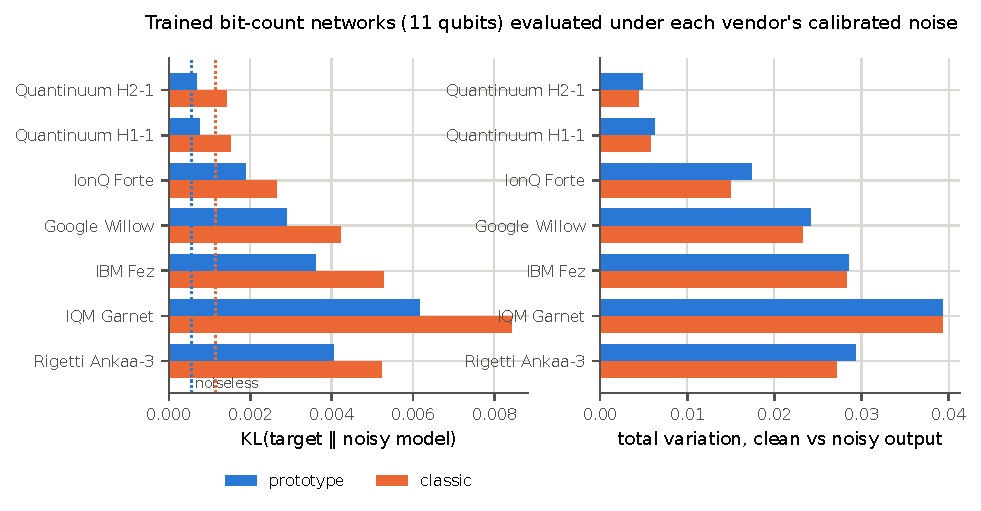
\includegraphics[width=\textwidth]{fig_bitcount_noise_devices}
\caption{The trained bit-count networks under each machine's noise model.  Left: KL to the
target (dotted lines: the noiseless values).  Right: how far the output distribution moved.
Rigetti's row models only its two-qubit error.  Run \run{bitcount\_noise/20260820T145335Z}.}
\label{fig:bitcount-noise-devices}
\end{figure}

\begin{figure}[t]
\centering
\begin{minipage}[t]{0.5\textwidth}\centering
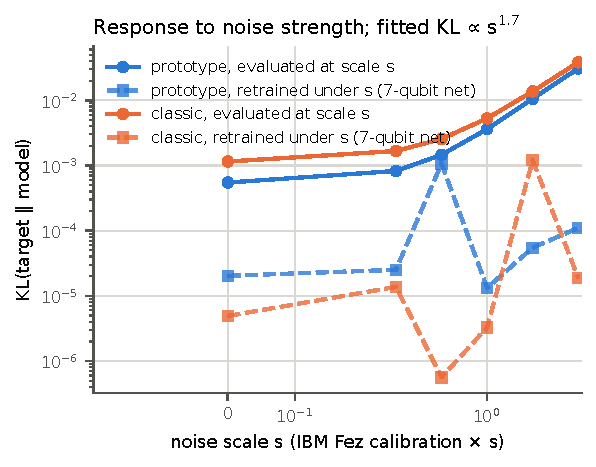
\includegraphics[width=\textwidth]{fig_bitcount_noise_scale}
\caption{Response to noise strength: IBM Fez's calibration scaled by $s$ (solid), and a
7-qubit network retrained with the scaled noise in the loop (dashed).  Same run.}
\label{fig:bitcount-noise-scale}
\end{minipage}\hfill
\begin{minipage}[t]{0.47\textwidth}\centering
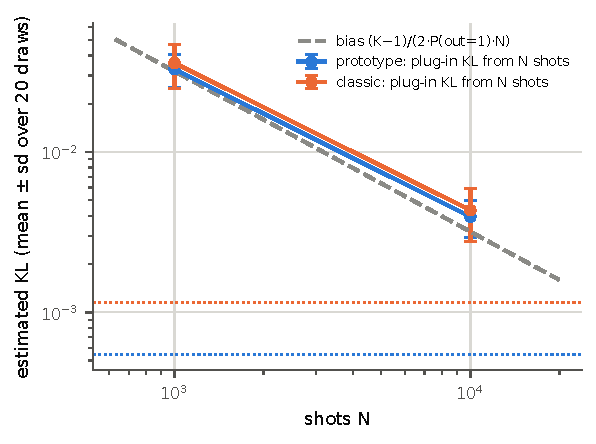
\includegraphics[width=\textwidth]{fig_bitcount_plugin_bias}
\caption{Estimating the KL from $N$ shots: the plug-in estimate sits above the true value by
$(K-1)/(2\,\Pout\,N)$, with $K=32$ bins and only $\Pout\approx 0.49$ of the shots usable.}
\label{fig:plugin-bias}
\end{minipage}
\end{figure}

\begin{figure}[t]
\centering
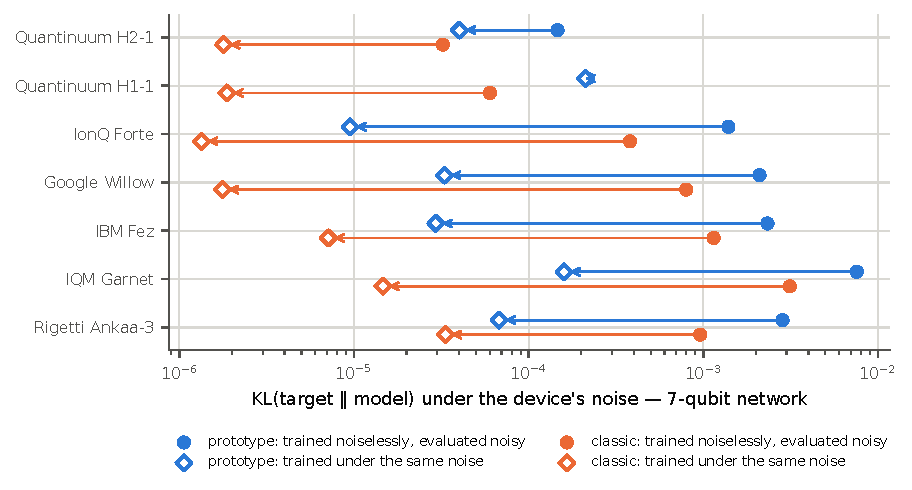
\includegraphics[width=0.9\textwidth]{fig_bitcount_noise_aware}
\caption{Noise-aware training (7-qubit bit-count network, three seeds): KL under each
machine's noise for parameters trained noiselessly (filled) and for parameters trained with the
same noise model in the loop (open), median of three seeds.}
\label{fig:bitcount-noise-aware}
\end{figure}

\subsection{Flappy Bird}
\label{sec:noise-flappy}

The Flappy controller is a thresholded activation, so what matters is not how far $\Pout$ moves
but whether it crosses $\tfrac12$.  Evaluated exactly under every preset on its $65\times65$
decision grid and then played for 20 held-out games (run
\run{flappy\_noise/20260820T154249Z}; \cref{fig:flappy-noise}, left), the controller \emph{still
plays perfectly on all seven machines}: only $1.5$--$4\,\%$ of the frames it actually visits are
decided differently, because the noise contracts every activation toward $\tfrac12$ by about the
same amount (mean $|\Delta P| = 0.002$--$0.018$) and so rarely changes the ordering
$P\gtrless\tfrac12$.  There is a factor of two of headroom: IBM Fez's noise scaled by $2$ leaves
$60\,\%$ of games perfect, by $4$ none (\cref{fig:flappy-noise}, right).

Shot noise is a different matter (\cref{fig:flappy-shot-noise}).  Re-deciding every frame from
$N$ measurements of the output qubit, the same controller wins no game at $N=1\,000$, $90\,\%$
at $4\,000$ and all at $10\,000$ on a noiseless simulator; on IBM Fez's model only $55\,\%$ at
$4\,000$.  The reason is the distribution of decision margins over the frames the agent plays:
median $\delta = 0.019$, tenth percentile $0.004$, first percentile $0.0002$ (right panel).  The
measured flip rate per frame agrees with the average of $\Phi(-2\delta\sqrt N)$ over that
distribution to $3\,\%$.  A deterministic shift of the boundary (gate noise) is tolerated far
past a stochastic one: Fez at scale $2$ decides $20\,\%$ of frames differently and still wins
$60\,\%$ of games; $1\,000$ shots decide only $8.5\,\%$ differently and win none.  A controller
that is re-rolled every frame is a jittery controller, and two or three unlucky frames in a row
are a collision.  Fine-tuning under Fez's noise for five sweeps changes nothing (the training
episodes already all survive, so the objective has no slope).

\begin{figure}[t]
\centering
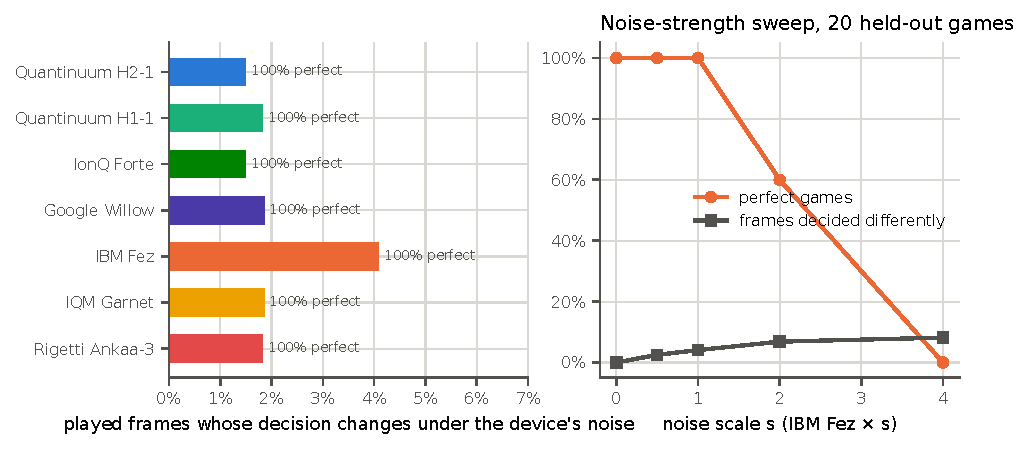
\includegraphics[width=\textwidth]{fig_flappy_noise}
\caption{Flappy under gate noise.  Left: fraction of played frames whose decision changes
under each machine's model; every machine still yields $100\,\%$ perfect games.  Right: IBM
Fez's noise scaled by $s$.  Run \run{flappy\_noise/20260820T154249Z}.}
\label{fig:flappy-noise}
\end{figure}

\begin{figure}[t]
\centering
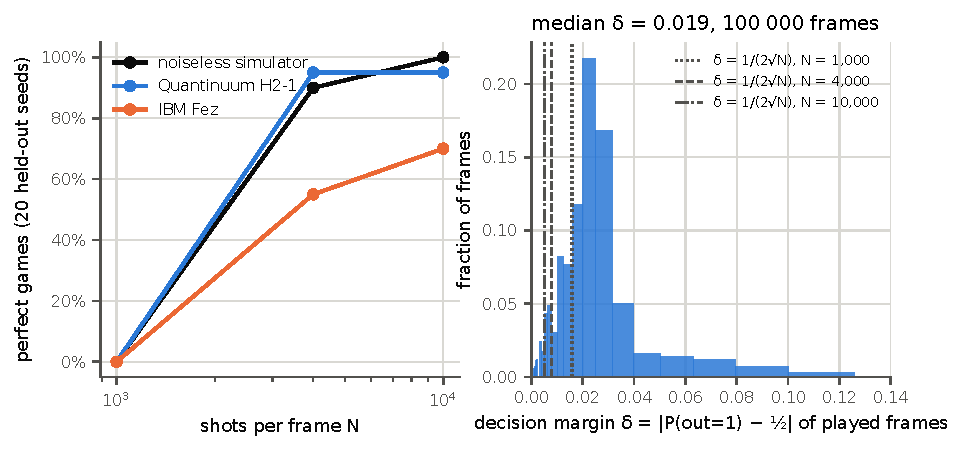
\includegraphics[width=\textwidth]{fig_flappy_shot_noise}
\caption{Flappy under shot noise.  Left: perfect games when every frame is decided from $N$
shots.  Right: distribution of the decision margin $\delta$ over the $100\,000$ frames the
noiseless controller plays; the vertical lines mark the margin that $N$ shots can just resolve.
Same run.}
\label{fig:flappy-shot-noise}
\end{figure}

\subsection{ECG and Iris (reduced run)}
\label{sec:noise-ecg-iris}

The ECG and Iris grids were run in a \emph{reduced} configuration only (run
\run{ecg\_iris\_noise/20260820T155618Z}): ECG on 8 test windows instead of 898 and two presets
instead of seven; Iris with 16 Monte-Carlo trajectories per evaluation instead of 2\,000 (per-outcome
standard error $\approx 12\,\%$), two presets, and perfect preparation of the dataset state
assumed.  The measured cost of the full grids --- 4--6 CPU-hours for ECG, 8 hours for Iris --- put
them outside the session's budget, and they were not run.  What the reduced run shows
(\cref{fig:ecg-iris-noise}) is indicative only: ECG denoising loses $-0.1$ to $+0.4$~dB under
Quantinuum H2-1 and $1.6$--$2.7$~dB (classic) under IBM Fez, while the prototype cells
\emph{gain} up to $3.8$~dB under Fez on eight windows --- a small-sample artefact, not a finding.
Iris keeps its $95\,\%$ accuracy under H2-1 and loses it under Fez ($64\pm44\,\%$ over two
trajectory seeds) for the prototype network, whose read-out is a conditional distribution over
4\,096 input strings and therefore directly exposed to probability leaking out of the 20-code
support.  One noisy sweep of ECG fine-tuning gains $2.7$~dB under Fez and $3.7$~dB noiselessly
--- it finishes the clean optimisation, it does not fold the channel in.

\begin{figure}[t]
\centering
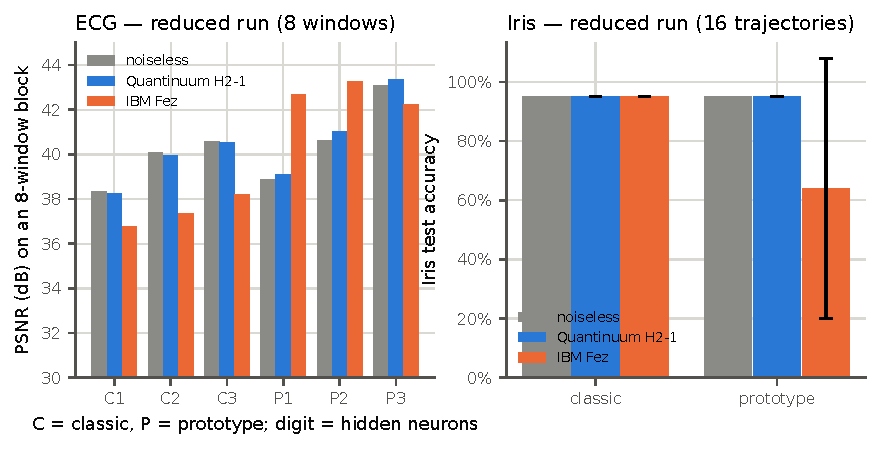
\includegraphics[width=\textwidth]{fig_ecg_iris_noise}
\caption{Reduced-configuration noise runs, quoted for the record.  Left: ECG PSNR on an
8-window block.  Right: Iris test accuracy from 16 trajectories (error bars: two trajectory
seeds).  Run \run{ecg\_iris\_noise/20260820T155618Z}.}
\label{fig:ecg-iris-noise}
\end{figure}

\section{What it takes to run this on a real machine}
\label{sec:hardware}

All numbers in this section are printed by \code{experiments/hardware\_plan.py} into
\run{hardware-plan/20260821T073211Z/numbers.md}; the script joins every calibration number
it uses to its provenance entry and refuses to run if one is missing.

\subsection{Compilation: the prototype network is the worst case for a lattice}
\label{sec:compile}

Every prototype neuron touches every input, so the network's two-qubit gates form a complete
bipartite graph between inputs and hidden qubits.  On an all-to-all machine (trapped ions) each
controlled rotation costs exactly two native two-qubit gates and nothing else: 24 for Flappy,
60 for bit-count.  On a lattice the compiler must insert SWAPs, three native gates each, to
bring non-neighbouring qubits together.  With our own router (greedy, no look-ahead) the
bit-count circuit needs 327 native two-qubit gates on IBM's heavy-hex lattice and 207 on a
square lattice, of which $82\,\%$ and $71\,\%$ are SWAP-borne (\cref{fig:entanglers}).  IBM's
own compiler does much better --- 97 gates at its optimisation level~2, $3.4\times$ fewer --- so
our router is a device-independent comparison instrument, not what one would submit.  Flappy's
circuit is 12.9\,µs long on Fez (1.56\,µs of which is readout) and 17.9\,ms on IonQ Forte, whose
gates take a millisecond.

\begin{figure}[t]
\centering
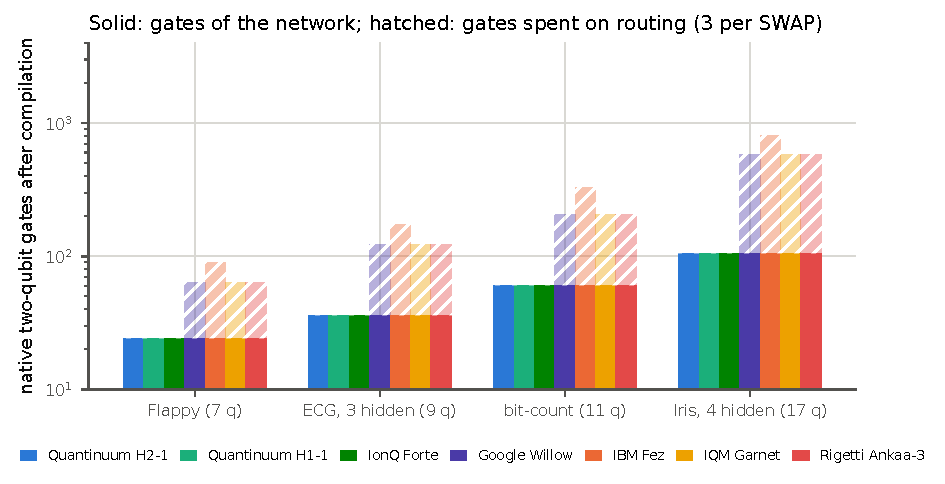
\includegraphics[width=\textwidth]{fig_hardware_entanglers}
\caption{Native two-qubit gates after compiling each network for each machine (our router;
log scale).  The all-to-all machines need only the network's own gates; the lattices spend most
of their budget on routing.  Run \run{hardware-plan/20260821T073211Z}.}
\label{fig:entanglers}
\end{figure}

\subsection{Expected fidelity}
\label{sec:fidelity}

\Cref{fig:fidelity} stacks the four factors of \cref{eq:fidelity} for the two smallest
circuits, with the exactly simulated total-variation distance between the compiled circuit run
clean and run under the machine's noise model next to each bar.  Flappy at 7 qubits is a
high-fidelity circuit on the trapped-ion machines ($F\approx 0.92$ on H2-1, $0.81$ on Forte),
marginal on Willow and Fez ($0.6$, $0.4$ with our router, $0.72$ with IBM's compiler), and poor on
Garnet ($0.18$).  Bit-count at 11 qubits is feasible on H-series ($0.81$) and Forte ($0.61$),
usable with IBM's compiler on Fez ($0.43$), and dead on Garnet ($0.004$), whose routed circuit
lasts $86\,\%$ of its $T_2$.  Two cautions.  The simulated distances of the \emph{compiled}
circuits ($0.03$ on H-series, $0.16$ on Forte, $0.43$ on Fez) are $5$--$15\times$ larger than
those of the uncompiled circuits in \cref{sec:noise-bitcount}: two native gates per controlled
rotation, resynthesised one-qubit gates and routing all cost.  And the vendors' two-qubit errors
are measured in isolation; IBM's own layered benchmark for Fez is $1.7\times$ worse than its
isolated gate error, so the lattice numbers are optimistic.

\begin{figure}[t]
\centering
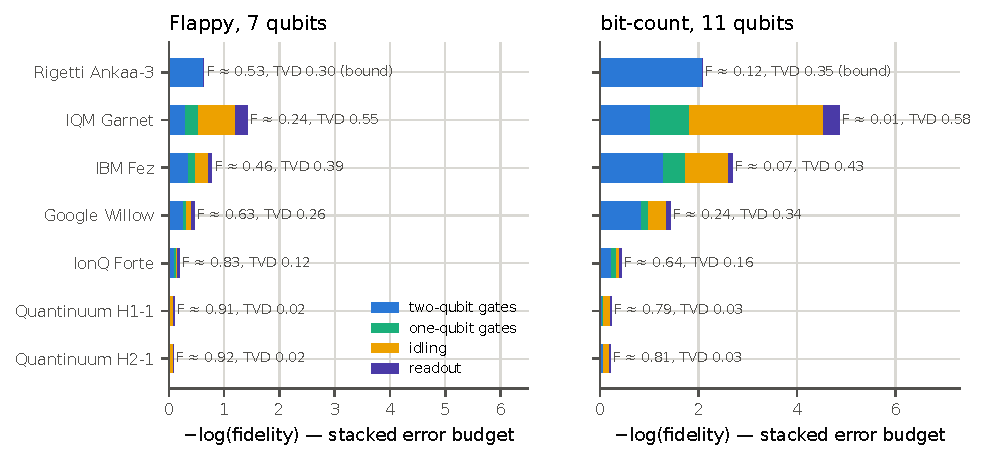
\includegraphics[width=\textwidth]{fig_hardware_fidelity}
\caption{Error budget per machine for the Flappy (left) and bit-count (right) circuits: the
stacked bars are $-\log$ of each factor of \cref{eq:fidelity}, so their total is $-\log F$;
the labels give $F$ and the simulated total-variation distance of the compiled circuit.
Quantinuum's idle term comes from its published memory error; Rigetti's is a bound (two-qubit
error only).}
\label{fig:fidelity}
\end{figure}

\subsection{Shots, time and money}
\label{sec:cost}

The shot budgets follow from \cref{sec:notation}.  An activation to $\pm 0.005$ needs
$10\,000$ shots.  The 32-bin bit-count histogram is estimated from the shots in which the
output fired ($\Pout = 0.487$ of them), and the plug-in KL is then biased upward by
$(K-1)/(2\cdot 0.487\cdot N) = 31.8/N$; reaching the trained model's $5.5\times10^{-4}$ needs
$58\,000$ shots, which we round to a $64\,000$-shot job.  The ECG denoiser's PSNR is capped by
shot noise at $10\log_{10}(4N)$: $2\,500$ shots per sample cap it at exactly $40$~dB, the
paper's Table~I value, and a $1\,800$-sample trace at $25\,000$ shots is $4.5\times10^7$ shots
--- ECG is a simulator experiment.  \Cref{fig:qpu-time} converts the circuit times to machine
time per job: milliseconds to two seconds on the superconducting machines, where the per-job
overhead dominates, but $72$\,s (Flappy) and $32$\,min (bit-count) on IonQ Forte, where the
circuit time does.  Prices (retrieved 20 August 2026; \cref{tab:cost}): a $4\,000$-shot Flappy
job costs about \$320 on Forte through Braket, \$6 on Garnet, $323$ Quantinuum credits
($\approx$\,\$4\,000 at the Azure plan rate), and is free on IBM's Open plan.  Training on
hardware is out of the question --- the paper's $2\,160$ evaluations at $64\,000$ shots are
$1.4\times10^8$ shots, $48$ days of Forte time or \$11\,M --- but fine-tuning the six output
angles ($90$ evaluations at $4\,000$ shots) is $1.8$ hours on Forte and about $45$ minutes on Fez.
Live Flappy play is equally out ($1\,500$ frames $\times$ $4\,000$ shots $\times$ $17.9$\,ms
$=30$ hours per episode on Forte); the falsifiable hardware observable is the activation map of
\cref{fig:flappy-policy} on a grid of observations, $16$ jobs.

\begin{table}[t]
\centering\small
\caption{Cost per job (numbers.md §cost).  IBM: \$1.60 per QPU second plus a 30\,s per-job
overhead (both assumptions, \cref{app:assumptions}); Quantinuum: the vendor's published credit
formula, converted at the Azure plan rate; Braket: published per-shot prices.}
\label{tab:cost}
\begin{tabularx}{\textwidth}{@{}l X l l@{}}
\toprule
Machine & model & Flappy, 4\,000 shots & bit-count, 64\,000 shots \\
\midrule
IBM Fez & \$1.60/s; 52\,ms resp.\ 1.8\,s of QPU & \$0.08 (\$48 with overhead) & \$2.85 (\$51) \\
IBM Open plan & 10 min per 28 days, free & \$0 & \$0 \\
Quantinuum H1/H2 & credits $=5 + (N_1 + 10N_2 + 5N_m)C/5000$ & 323 credits $\approx$ \$4\,030 & 11\,920 credits $\approx$ \$149\,000 \\
IonQ Forte (Braket) & \$0.30 + \$0.08/shot & \$320 & \$5\,120 \\
IQM Garnet (Braket) & \$0.30 + \$0.00145/shot & \$6.10 & \$93 \\
\bottomrule
\end{tabularx}
\end{table}

\begin{figure}[t]
\centering
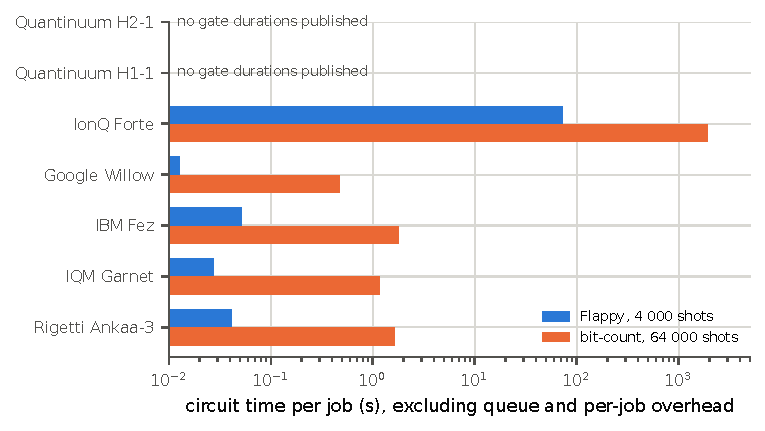
\includegraphics[width=0.75\textwidth]{fig_hardware_qpu_time}
\caption{Machine time per job, from the compiled circuit's duration (our router; readout
included where published).  Quantinuum publishes no durations.}
\label{fig:qpu-time}
\end{figure}

\subsection{Recommendation}
\label{sec:recommendation}

Run the 7-qubit Flappy activation map first: on IBM's free plan to debug the pipeline (readout
calibration, then zero-noise extrapolation by gate folding, both validated offline against the
noise model first), then on IonQ Forte for the confirmation (\$1\,300 for a $4\times4$ grid at
$1\,000$ shots), and on Quantinuum H2-1 for the headline number if an allocation exists.  The
bit-count histogram is feasible on H-series and Forte as a \emph{shape} demonstration but not as
a KL comparison (device error puts the KL floor at $10^{-2}$--$10^{-1}$, two orders above the
simulated $5.5\times10^{-4}$).  Iris is out of reach: loading the dataset state needs thousands
of two-qubit gates ($8\,166$ dense, $\approx 1\,440$ exploiting sparsity \cite{sbm,plesch,gleinig}),
giving a best-case fidelity near $0.2$ before the network runs.  Four things the code still
lacks for a live submission are listed in the repository's hardware plan (credentials, the
vendors' own routing, asynchronous job handles, readout-unfolding and folding utilities).

\section{The shot-noise programme}
\label{sec:shots}

\Cref{sec:noise} found that, at today's published error rates, what limits a hardware
demonstration of these networks is not gate error but the number of measurements.  Two
mechanisms were identified: a thresholded controller whose decisions sit close to its threshold
flips at a rate set by $\Phi(-2\delta\sqrt N)$; and a histogram loss estimated from $N$ shots is
biased upward by $(K-1)/(2\,\Pout\,N)$ and discards the half of the shots in which the output
did not fire.  Six remedies were proposed; this section reports the three we implemented and
tested (\cref{tab:shots-summary}).  All runs are noiseless state-vector simulations plus
sampling, minutes each.

\begin{table}[t]
\centering\small
\caption{The shot-noise programme: what was tried and what came out.  Items 4--6
(joint-distribution loss or amplitude amplification to use all shots; bias-corrected KL
estimators; amplitude estimation) are designed but not implemented.}
\label{tab:shots-summary}
\begin{tabularx}{\textwidth}{@{}l X X@{}}
\toprule
Remedy & Mechanism & Outcome \\
\midrule
1. Margin-aware training & add a penalty for frames whose margin $\delta$ is below $m=0.1$ &
\textbf{negative}: margins of this network barely move; play under shot noise gets worse \\
2. Common random numbers & evaluate the two finite-difference probes on the same measurement
randomness (maximal coupling) & derivative variance $\div 3$ at our reproduction's step ($c=0.2$), $\div 12$--$22$
at small steps; sampled training improves at $N\le 4\,000$ but stays $10\times$ above the
exact-probability result, consistent with the bias of the loss itself \\
3. Sequential decisions & Wald's sequential test on the sign of $\Pout-\tfrac12$ per frame &
\textbf{positive}: $100\,\%$ perfect games at about $2\,200$ shots/frame, $4.6\times$ fewer than
the fixed budget that achieves the same \\
\bottomrule
\end{tabularx}
\end{table}

\subsection{Margin-aware training (negative result)}
\label{sec:margin}

The idea: if the controller could be trained so that every frame it visits has
$\delta\ge 0.1$ instead of the median $0.019$, the shots needed per frame would fall by
$(0.1/0.019)^2\approx 25\times$, at no cost on a noiseless simulator.  We added to the training
objective a penalty of $w\times 0.01\times\max(0, 1-\delta/m)$ per played frame --- a fraction
$w<1$ of the $0.01$ reward for surviving that frame, so that surviving a frame is always worth more
than dying confidently --- and fine-tuned the trained controller for 25 sweeps with $m = 0.1$
and $w\in\{0.25, 0.5, 1\}$ (run \run{flappy\_shots/20260821T084601Z}).  A first attempt with a
\emph{mean} hinge of weight 20, trained from scratch, had collapsed to a policy that died in 30
frames with perfectly confident decisions (run \run{…T075048Z}): any penalty that can outweigh
the per-frame reward selects for dying early, which is why the per-frame form is necessary.

\Cref{fig:flappy-shots} (left) shows the outcome: the margin quantiles hardly move (median
$0.019\to0.021$--$0.024$, tenth percentile $0.004\to0.006$).  All three fine-tuned controllers
still play perfectly on exact probabilities, but under shot noise they play \emph{worse} than the
original at $w\ge 0.5$ ($50\,\%$ and $80\,\%$ perfect games at $10\,000$ shots against
$100\,\%$).  The explanation is in \cref{fig:flappy-policy}: the activation is a smooth surface
over the two observations, and the near-boundary frames are those in which the bird hovers at
the boundary --- a property of the game's dynamics, not of the surface's steepness.  Penalising
them moves the boundary rather than steepening it, and a moved boundary is a less stable
controller.  A 17-parameter network has no spare capacity to steepen its surface.  We record
the remedy as not working for this network.

\begin{figure}[t]
\centering
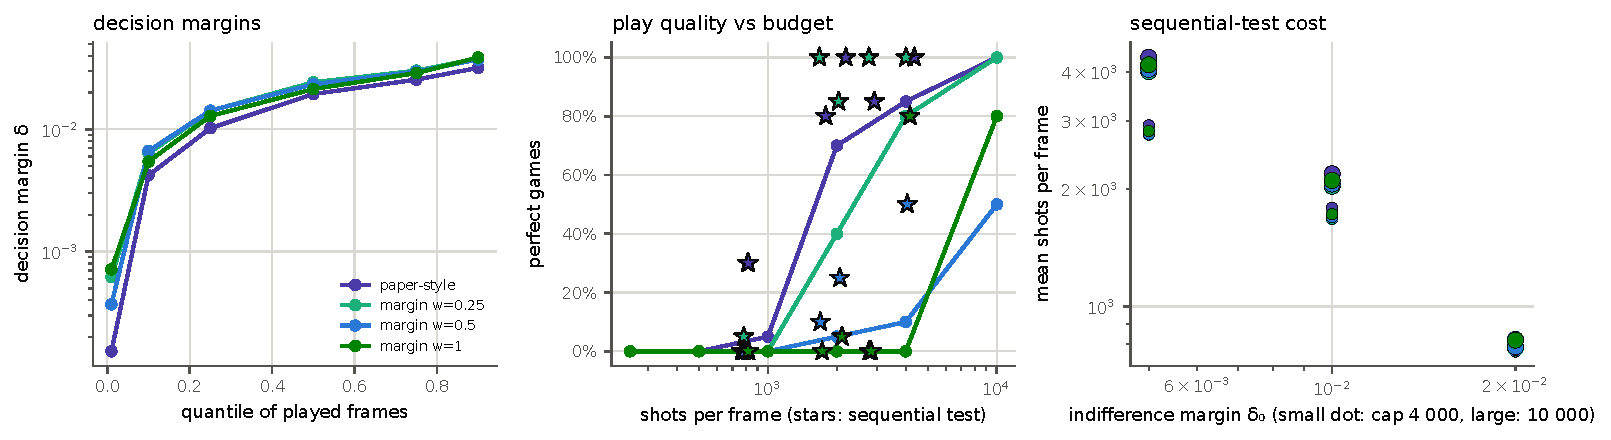
\includegraphics[width=\textwidth]{fig_flappy_shots_programme}
\caption{Flappy under shot noise, remedies 1 and 3.  Left: decision-margin quantiles of the
frames played by the original and the three margin-aware controllers.  Middle: perfect games
against shots per frame for a fixed budget (lines) and for the sequential test (stars, at the
mean shots it actually spent).  Right: mean shots per frame of the sequential test against its
indifference margin $\delta_0$.  Run \run{flappy\_shots/20260821T084601Z}.}
\label{fig:flappy-shots}
\end{figure}

\subsection{Common random numbers for the finite-difference optimiser}
\label{sec:crn}

\paragraph{Mechanism.}
The paper's optimiser estimates a slope as $(f(x+c)-f(x-c))/2c$.  If each probe is estimated
from $N$ independent shots with variance $\sigma^2$, the slope has variance $\sigma^2/2c^2$ ---
at our reproduction's $c=0.2$ that is $12.5\sigma^2$, which is why finite differences on a
sampling backend stall.  If the two probes are instead computed from the \emph{same} random draws, the
noise largely cancels.  The standard way (feeding the same uniform random numbers to the inverse
cumulative distribution of both probes) turned out to give only a $1.3\times$ reduction here,
because a parameter change moves probability between distant bit strings and so shifts every
later bin boundary.  What works is the \emph{maximal coupling} \cite{lindvall}: sample the first
probe, then for the second keep each shot's outcome $i$ with probability
$\min(1, p_{\mathrm{new}}(i)/p_{\mathrm{ref}}(i))$ and redraw it otherwise from the excess
$(p_{\mathrm{new}}-p_{\mathrm{ref}})_+$.  The second sample has exactly the right distribution,
and only $N\cdot\TV(p_{\mathrm{new}},p_{\mathrm{ref}})$ shots change --- the fewest any coupling
can achieve.  Since $\TV\propto c$, the difference of the two estimates has variance $O(c/N)$ and
the slope, after division by $2c$, has variance $O(1/(cN))$ instead of $O(1/(c^2N))$: a gain of
order $1/c$.  Coupling reduces the variance of the slope; it does not remove the bias of a
non-linear loss such as the plug-in KL.  On hardware the analogue is to interleave the $\pm c$ circuits in one job so they
share the same drift.

\paragraph{Measurement.}
\Cref{fig:crn} measures the variance of one slope of the bit-count loss at $400$ shots per
probe: the reduction is $\times 2$--$3$ at $c=0.2$--$0.4$ and $\times 22$--$29$ at $c=0.025$--$0.05$,
as the $1/c$ scaling predicts, and both estimates are unbiased for the exact slope.
\Cref{fig:sampled-training} then trains the 11-qubit bit-count network with our reproduction's
schedule (the paper publishes none) on a sampling backend (run \run{bitcount\_shots/20260821T084558Z}): at $N=1\,000$
shots per evaluation the exact KL after 20 sweeps improves from $0.080$ to $0.059$ with common
random numbers, at $4\,000$ from $0.050$ to $0.014$, and at $16\,000$ the two are within the
seed-to-seed spread ($0.029$ vs $0.033$).  All of them remain an order of magnitude above the
exact-probability result ($0.0009$).  The right panel suggests why: the \emph{loss} is the plug-in
KL of a 32-bin histogram from about $N/2$ usable shots, biased by $31.8/N$, and the reached KL
tracks one to three times that bias.  This is consistent with the estimator, not the optimiser,
being what now limits sampled training, but three seeds (one of which stalls at $0.014$ even on
exact probabilities) cannot separate the two; a bias-corrected or joint loss under paired
initialisations is the test, and it has not been run.  Our step schedule ($c_0 = 0.2$ decaying
only to $0.15$ over 20 sweeps) also keeps the optimiser in the regime where the reduction is
smallest.

\begin{figure}[t]
\centering
\begin{minipage}[t]{0.47\textwidth}\centering
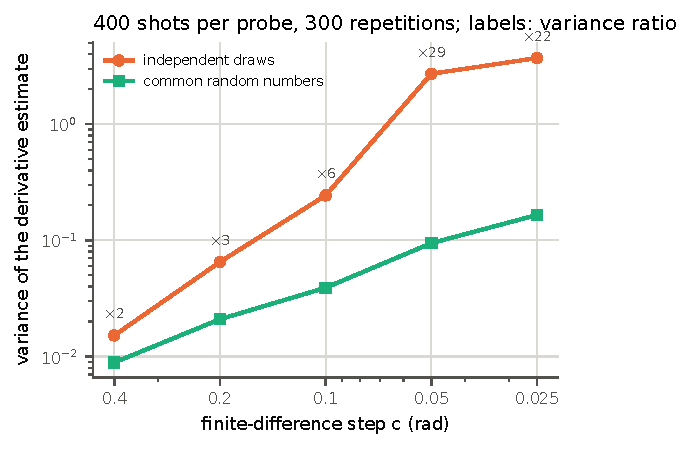
\includegraphics[width=\textwidth]{fig_crn_variance}
\caption{Variance of the finite-difference slope of the bit-count loss at 400 shots per
probe, with independent draws and with maximally coupled draws; labels give the ratio.}
\label{fig:crn}
\end{minipage}\hfill
\begin{minipage}[t]{0.5\textwidth}\centering
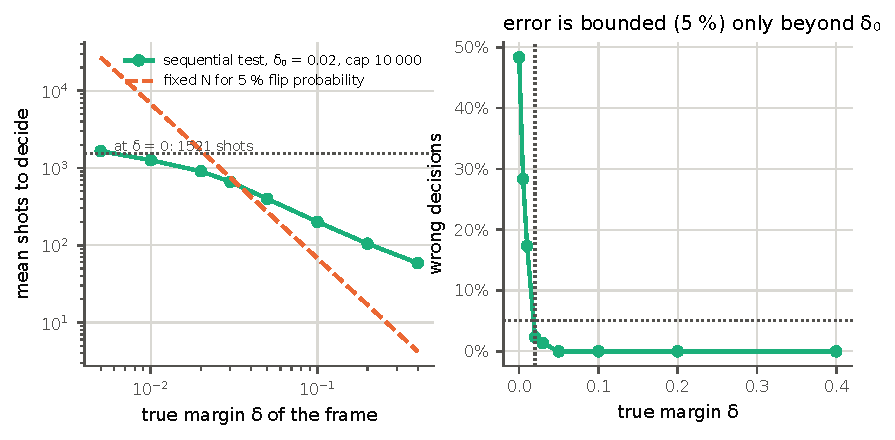
\includegraphics[width=\textwidth]{fig_sprt_cost}
\caption{The sequential test ($\delta_0=0.02$, $5\,\%$ error bounds, cap $10\,000$): mean
shots to decide a frame against its true margin (left), and its error rate (right), which is
bounded only beyond $\delta_0$.}
\label{fig:sprt-cost}
\end{minipage}
\end{figure}

\begin{figure}[t]
\centering
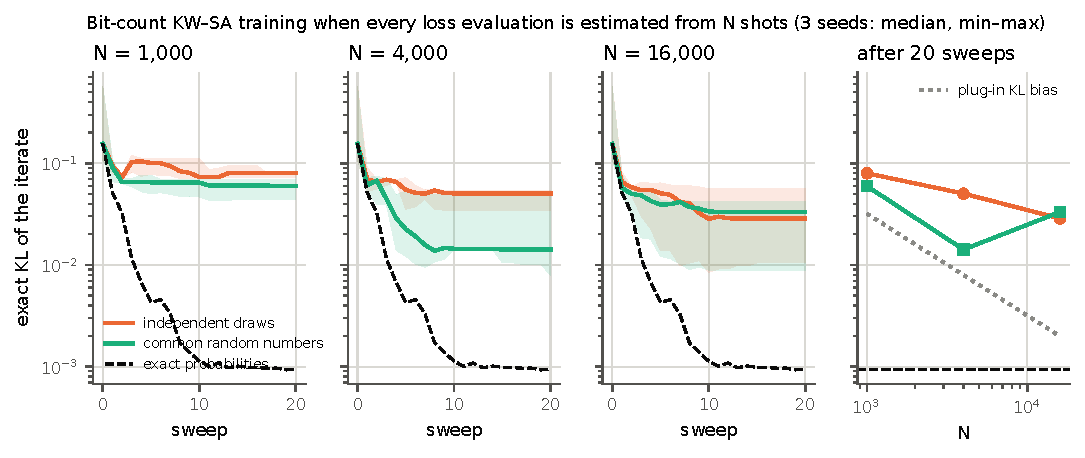
\includegraphics[width=\textwidth]{fig_bitcount_sampled_training}
\caption{Bit-count training when every loss evaluation is estimated from $N$ shots (three
seeds; median and range), with and without common random numbers, against training on exact
probabilities.  Right: the exact KL reached after 20 sweeps against $N$, with the plug-in bias
of the loss for comparison.  Run \run{bitcount\_shots/20260821T084558Z}.}
\label{fig:sampled-training}
\end{figure}

\subsection{Sequential decisions (positive result)}
\label{sec:sprt}

\paragraph{Mechanism.}
A fixed budget of $N$ shots per frame wastes most of them: a frame with $\delta = 0.3$ is decided
correctly after a dozen shots.  Wald's sequential probability ratio test \cite{wald} between the
hypotheses ``$\Pout = \tfrac12+\delta_0$'' and ``$\Pout = \tfrac12-\delta_0$'' draws shots in
blocks, after $n$ shots with $k$ ones computes the log-likelihood ratio
$\Lambda = (2k-n)\log\frac{1+2\delta_0}{1-2\delta_0}$, and stops as soon as
$\Lambda\ge\log\frac{1-\beta}{\alpha}$ (flap) or $\Lambda\le\log\frac{\beta}{1-\alpha}$ (do not
flap), up to a cap $N_{\max}$ after which the majority decides.  For a frame whose true margin
exceeds $\delta_0$ the error probability is at most about $\alpha$ ($=\beta=5\,\%$ here); for a
frame nearer the boundary than $\delta_0$ the test is slow and its error is not bounded
(\cref{fig:sprt-cost}).

\paragraph{Measurement.}
Played on the same 20 held-out games (\cref{fig:flappy-shots}, middle and right;
\cref{tab:sprt}), the sequential rule with $\delta_0 = 0.01$ and cap $10\,000$ wins \emph{every}
game at a mean of $2\,191$ shots per frame --- the fixed budget needs $10\,000$ for the same
result, $4.6\times$ more --- and with $\delta_0 = 0.005$ and cap $4\,000$ it matches the fixed
$4\,000$-shot result ($85\,\%$) at $2\,916$.  Setting $\delta_0$ at the median margin ($0.02$) fails
($30\,\%$ perfect at $820$ shots): the frames that decide a game are the near-boundary ones, and
the indifference margin must sit below \emph{their} margins (the tenth percentile, $0.004$--$0.006$),
not the typical one.  The rule needs no change to the network, no retraining, and is what one
would submit to a machine that supports mid-circuit decisions or, more simply, adaptive batch
sizes per frame.

\begin{table}[t]
\centering\small
\caption{Flappy, original controller, 20 held-out games: fixed shot budgets against the
sequential test ($\alpha=\beta=0.05$).  ``Flips'' are frames decided differently from the
exact rule.  Run \run{flappy\_shots/20260821T084601Z}.}
\label{tab:sprt}
\begin{tabular}{@{}l S[table-format=3.0] S[table-format=3.0] S[table-format=2.2] S[table-format=5.0]@{}}
\toprule
Decision rule & {perfect games (\%)} & {median pipes} & {flips (\%)} & {mean shots/frame} \\
\midrule
fixed $N = 1\,000$ & 5 & 23 & 8.36 & 1000 \\
fixed $N = 2\,000$ & 70 & 110 & 7.40 & 2000 \\
fixed $N = 4\,000$ & 85 & 110 & 6.09 & 4000 \\
fixed $N = 10\,000$ & 100 & 110 & 4.47 & 10000 \\
sequential, $\delta_0 = 0.02$, cap $10\,000$ & 30 & 88 & 7.19 & 822 \\
sequential, $\delta_0 = 0.01$, cap $4\,000$ & 80 & 110 & 6.12 & 1790 \\
sequential, $\delta_0 = 0.005$, cap $4\,000$ & 85 & 110 & 5.98 & 2916 \\
sequential, $\delta_0 = 0.01$, cap $10\,000$ & 100 & 110 & 5.06 & 2191 \\
sequential, $\delta_0 = 0.005$, cap $10\,000$ & 100 & 110 & 4.50 & 4358 \\
\bottomrule
\end{tabular}
\end{table}

\section{What we learned}
\label{sec:learnings}

\begin{enumerate}[leftmargin=*,itemsep=2pt]
\item \textbf{The paper's central claims reproduce.}  The prototype neuron's activation surface,
the bit-count histogram and its convergence, the Iris overfitting contrast, perfect Flappy play
(on our clone) and the ECG denoising numbers (within 2~dB on a different signal) all come out of
a clean-room implementation.  What does not: the weight picture of Fig.~9 --- scored over 20
seeds against a criterion fixed in advance, the prototype layer does cover more of the data than
the classic one, but an untrained prototype layer already does, so the effect is the
architecture's rather than training's, and the trained angles do not decode to data patterns
(\cref{sec:iris}) --- and --- once the paper's own ECG recording reached us and removed
the signal as an excuse --- the upper half of Table~I, where our two- and three-neuron prototype
cells fall $2.5$--$3.2$~dB short ($2.2$--$3.8$~dB on the full recording) while the one-neuron cell reproduces with a \emph{larger}
prototype advantage than the paper's (\cref{sec:ecg}).  The iterative baseline of Fig.~6 was a second such failure until
we noticed that we had been grading it with the wrong quantity: a scheme that trains one input at
a time moves the per-input activations, not the superposition distribution of
\cref{eq:model-distribution}, and because the prototype block leaves the input register entangled
with the hidden qubits the two are genuinely different.  In its own observable the baseline
reaches the paper's $\approx 10^{-3}$ on four seeds of six (\cref{sec:bitcount}); only the unit
of the paper's ``iteration'' is still assumed.  Grade a scheme in the observable it optimises.

\item \textbf{Reading figures is part of reproduction.}  The bit-count target
($(\text{ones}+1)/112$), the Iris label weighting ($(\ell+1)^2$) and the angle encoding
($\theta = 2\arcsin\sqrt s$, from a printed gate angle in the companion paper) all had to be
read off figures; each was then confirmed to the figure's precision.  Where a figure was
over-read --- the Iris split ratio ``justified'' by bar counts --- an independent review caught
it and the justification was withdrawn (\cref{sec:iris}).

\item \textbf{The prototype network's advantage under noise is inherited, not intrinsic.}
Prototype and classic networks have the same two-qubit gate count and the noise displaces both
by the same amount; the prototype wins under noise because it fits better without noise.

\item \textbf{Gate noise at published levels is not the obstacle for these networks; shots
are.}  Every 7--11-qubit network survives every vendor's calibrated noise model with a
qualitatively intact result.  The Flappy controller needs $10^4$ shots per frame with a fixed
budget; the bit-count loss is biased by $31.8/N$.  The one remedy that pays now is a sequential
measurement rule ($4.6\times$ fewer shots, no retraining); margin-aware training does not work
for a 17-parameter network; common random numbers reduce the optimiser's noise by $1/c$ but
leave the estimator's bias, which is the likely (untested) limit of sampled training.

\item \textbf{Compiled circuits are $5$--$15\times$ more noise-sensitive than logical ones.}
Two native gates per controlled rotation, resynthesised single-qubit gates and routing on a
lattice all cost; a complete-bipartite network is the worst case for a lattice, and the vendor's
own compiler must be used for any superconducting submission.  Trapped ions are the natural home
of this architecture; their price is circuit time (milliseconds per shot).

\item \textbf{An optimiser that keeps a stale incumbent turns a harmless change into a
negative result.}  The ``rotating seeds break training'' finding of the first session was an
artefact of comparing losses measured on different episode batches; re-scoring the incumbent
restores $25/25$ perfect games.  Any non-stationary objective (mini-batches, hardware drift) needs
this.

\item \textbf{Penalties must be priced in the currency of the reward.}  A margin hinge that
could outweigh the per-frame survival reward produced a confidently dead controller; the
per-frame form below the per-frame reward cannot.  The same arithmetic applies to any shaping
term.

\item \textbf{Provenance has to be mechanical.}  The first hardware plan contained a dozen
wrong numbers --- a state-preparation gate count off by a factor of two, a sentence with its
inequality reversed, costs computed by hand.  The fix was a script that emits every number and
refuses to run if any calibration input lacks a source; the report now quotes only that script.
\item \textbf{A read-out calibrated on the evaluated set is transductive.}  The Iris labels are
rounded after one overall scale is fitted; fitted on the test set itself (no test labels are
used), it makes a flower's label depend on which other flowers are evaluated with it: removing
the 13 test flowers that carry three ambiguous codes changed the labels of most of the rest
($94\,\% \to 39\,\%$ on one seed).  Only the 20-seed sweep exposed it; one seed would not have.
Calibrate on the training data, state the pass criterion before running the seeds --- and when a
score is a $z$-score against each model's own baseline, do not read it as a comparison between
the models (a review caught us doing exactly that).
\end{enumerate}

\paragraph{Not done, and why.}
Noise-aware training of the 11-qubit bit-count network (13 hours for its grid) and the full
ECG/Iris noise grids (4--8 hours) exceeded the session's compute ceiling and were not run;
their per-cell costs are recorded so that a future session can decide.  Items 4--6 of the
shot-noise programme --- a loss that uses all shots, bias-corrected estimators, and amplitude
estimation --- are designed but not implemented; item 4 is the natural next step, since the
estimator bias is what now limits sampled training.  Nothing has been submitted to a quantum
computer; the plan of \cref{sec:recommendation} is ready to be.


\appendix
\section{Choices the paper leaves open}
\label{app:assumptions}

Each entry is marked \code{[ASSUMPTION]} at the place in the code where it enters.

\begin{description}[leftmargin=1.2em,style=nextline,itemsep=2pt]
\item[Optimiser schedule (\cref{sec:kwsa}).]  Step sizes $a_n = a_0/(n+1)^{0.602}$,
difference step $c_n = c_0/(n+1)^{0.101}$, geometric cooling; one iteration is a coordinate
sweep.  Bit-count: $a_0 = 20$, $c_0 = 0.2$, $T_0 = 0.02$, cooling $0.7$, 20 sweeps.  Flappy:
$a_0 = 0.4$, $c_0 = 0.25$, $T_0 = 0.05$, cooling $0.9$, 25 sweeps after 300 random restarts.
Iris: $a_0 = 2$, decay exponent $0.3$, $c_0 = 0.1$, 40 sweeps.  ECG: 100 sweeps with restarts.
\item[Iterative baseline (\cref{sec:bitcount}).]  One optimiser sweep on the squared error of one
random input per iteration; the paper does not describe its scheme.
\item[Angle encoding (\cref{eq:encoding}).]  $\theta = 2\arcsin\sqrt s$, pinned by a printed
angle in \cite{snn}; $\theta = \pi s$ tested as an ablation.
\item[KL regularisation.]  The model probability is floored at $10^{-12}$ inside the logarithm.
\item[Iris (\cref{sec:iris}).]  Stratified one-third training split; flowers sharing a code are
merged and their labels averaged; the KL is normalised over all 4\,096 input strings (restricting
it to the dataset's codes lets the network exploit interference between examples and reach a
training loss of $10^{-5}$ while reading out at chance); label weight $\propto(\ell+1)^2$ read
from Fig.~8; labels predicted by nearest rounding of the read-out weight.
\item[Flappy (\cref{sec:flappy}).]  Our own clone: 288$\times$512 screen, flap impulse $-7$, gap
120, pipe spacing 180, gravity 1 (the classic constants are unplayable by a memoryless two-feature
policy); reward 0.01 per frame plus 1 per pipe, tracking term $|{\rm height}-{\rm gap}|$ with
weight 1; 5 training episodes of 1\,500 frames, 20 held-out seeds 5--24, 5\,000-frame cap (110
pipes); decisions cached on a $65\times65$ grid of observations.
\item[ECG (\cref{sec:ecg}).]  Synthetic McSharry-form signal tuned to Fig.~13 and MIT-BIH
record 100; Gaussian noise $\sigma = 0.02$; mirror-padded edges; first half train, second half
test; PSNR with $R = $ range of the clean signal; SSIM in a 7-sample sliding window.
\item[Noise model (\cref{sec:devices}).]  Depolarising at the vendor's average gate error,
relaxation during gates and as-soon-as-possible idling, readout confusion; median values where
vendors publish per-qubit tables; no crosstalk (no vendor publishes a usable number); where a
vendor publishes nothing for a channel it is modelled as error-free and flagged.  Quantinuum's
idle error is charged as $(1-m)^{n_{\rm qubits}\cdot{\rm depth}}$ from its memory error per
depth-1 time; IQM's and Rigetti's unpublished one-qubit gate durations are set to 40\,ns.
\item[Fidelity estimate (\cref{eq:fidelity}).]  First-order product of per-gate survival
probabilities; readout factor $(1-(p_{01}+p_{10})/2)^n$.
\item[Costs (\cref{sec:cost}).]  IBM \$1.60 per QPU second (2022 launch figure, corroborated by
a secondary \$96/min report) plus 30\,s per-job overhead; Quantinuum \$12.5 per credit (Azure
Standard plan divided by its allotment); Braket and Azure per-shot prices as retrieved on
20 August 2026; Quantinuum's credit formula with $N_m = 2\times$ qubits.
\item[State preparation (\cref{sec:recommendation}).]  Dense counts $2^{n+1}-2n-2$ \cite{sbm} and
$\approx\tfrac{23}{24}2^n$ \cite{plesch}; sparse leading term $k\cdot n$ with $k=120$ training
flowers \cite{gleinig}.
\item[Shot-noise programme (\cref{sec:shots}).]  Margin penalty $w\cdot 0.01\cdot\max(0,1-\delta/m)$
per frame with $m=0.1$; sequential test with $\alpha=\beta=0.05$, blocks of 20 shots; common
random numbers by maximal coupling to the first probe of each coordinate.
\end{description}

\section{Provenance of the calibration data}
\label{app:provenance}

Every calibration number used in \cref{sec:noise,sec:hardware} is stored in a device file
(\code{src/ptqnn/noise/devices/*.toml}) together with a \code{[[provenance]]} block per field:
the source URL, the kind of source (vendor calibration page, vendor paper, third-party
calibration snapshot), the retrieval date and a verbatim quotation of the sentence or table
row the number was read from.  The hardware-plan script joins these blocks to every field it
reads and fails if any is missing; the full join (one row per device and field, with quotations)
is the file \code{numbers.md} of run \runpath{hardware-plan/20260821T084554Z}, section
``provenance''.  The sources, in
brief:

\begin{description}[leftmargin=1.2em,style=nextline,itemsep=2pt]
\item[IBM Fez (Heron r2).]  One coherent calibration snapshot, backend version 1.2.8 of
2025-02-26, shipped as \code{props\_fez.json} inside \code{qiskit-ibm-runtime}'s fake provider;
medians over 156 qubits and 352 directed CZ edges computed by us from that table.  The file
records the same chip drifting between CZ error $2.85\times10^{-3}$ (2024-07) and
$3.90\times10^{-3}$ (2025-02).
\item[Quantinuum H1-1, H2-1.]  The vendor's performance-validation page
(\url{https://docs.quantinuum.com/systems/user_guide/hardware_user_guide/performance_validation.html}):
mean two-qubit and one-qubit infidelities, SPAM error, and ``Memory Error per Depth-1 Circuit
Time''; no gate durations and no $T_1$/$T_2$ are published.
\item[IonQ Forte.]  The vendor's published specification (average gate fidelities, gate
durations, $T_1 = 55$\,s, $T_2 = 1$\,s).
\item[Google Willow.]  The supplementary information of the Willow paper
(\emph{Nature}, 2024): single- and two-qubit gate errors, coherence times, cycle time.  The
machine is not publicly accessible; the preset exists for simulation only.
\item[IQM Garnet.]  Vendor data for gate errors and readout; $T_1$ and $T_2$ (echo) from a
third-party calibration snapshot (two epochs recorded, December 2025 and March 2026), with the
caveat that $T_2$ without echo is $\approx 8.5$\,µs.
\item[Rigetti Ankaa-3.]  Only the two-qubit (iSWAP) error $10^{-2}$ is published for the
universal gate; the $99.5\,\%$ headline refers to the fSim gate.  No one-qubit error, readout
error, $T_1$ or $T_2$.
\end{description}

The per-field table is not reproduced here --- it runs to some sixty rows with quotations ---
but it is the ground truth the numbers in this document rest on, and it is a single command
away: \code{uv run python experiments/hardware\_plan.py}.

\paragraph{One input that is not calibration data: the ECG recording.}
The ECG experiment of \cref{sec:ecg} also runs on the paper's own recording, sent to us by
B.~Rosenhahn by e-mail on 21 August 2026 as two MATLAB files.  They are the authors' data and are
not redistributed with this repository; instead the loader (\code{-{}-source mailed}) writes their
SHA256 digests into the \code{meta.json} of every run that uses them, so a run directory
identifies the input exactly without carrying it:

\begin{description}[leftmargin=1.2em,style=nextline,itemsep=2pt]
\item[\code{ecgfilteredData.mat} --- the clean trace.]
\code{9ed65523b30e588012dba0ece34e8d0bb6951254357cf0757ef1692b7439b456}
\item[\code{ecgnoiseData.mat} --- the noisy trace, already clipped to {$[0,1]$}.]
\code{cc94548d1c40b63b597b532edbf0bd198ac3a12ac9253d0efc4b40255d0753b9}
\end{description}

\noindent Runs \run{ecg/20260918T132924}, \run{ecg/20260925T153739Z-mailed1800} and
\run{ecg/20260925T165741Z-mailedfull} record both digests together with the sender and date.


\begin{thebibliography}{9}
\bibitem{ptqnn} B.~Rosenhahn and C.~Hirche, \emph{Prototype Learning for Quantum Neural
Networks}, manuscript \texttt{QPrototypeLearning-5.pdf} (2026).  Figure and equation numbers
cited as ``Fig.~5'', ``Eq.~(4)'' refer to this manuscript.
\bibitem{snn} B.~Rosenhahn, T.~J.~Osborne and C.~Hirche, \emph{Stochastic Neural Networks for
Quantum Devices}, arXiv:2602.22241 (2026).
\bibitem{kw} J.~Kiefer and J.~Wolfowitz, Stochastic estimation of the maximum of a regression
function, \emph{Ann.\ Math.\ Stat.}\ \textbf{23}, 462 (1952).
\bibitem{spall} J.~C.~Spall, \emph{Introduction to Stochastic Search and Optimization}, Wiley
(2003), \S6 (gain-sequence exponents $0.602$ and $0.101$).
\bibitem{wald} A.~Wald, Sequential tests of statistical hypotheses, \emph{Ann.\ Math.\ Stat.}\
\textbf{16}, 117 (1945).
\bibitem{lindvall} T.~Lindvall, \emph{Lectures on the Coupling Method}, Wiley (1992), \S I.2
(the maximal coupling).
\bibitem{nielsen} M.~A.~Nielsen, A simple formula for the average gate fidelity of a quantum
dynamical operation, \emph{Phys.\ Lett.\ A} \textbf{303}, 249 (2002).
\bibitem{sbm} V.~V.~Shende, S.~S.~Bullock and I.~L.~Markov, Synthesis of quantum-logic circuits,
\emph{IEEE Trans.\ CAD} \textbf{25}, 1000 (2006).
\bibitem{plesch} M.~Plesch and \v{C}.~Brukner, Quantum-state preparation with universal gate
decompositions, \emph{Phys.\ Rev.\ A} \textbf{83}, 032302 (2011).
\bibitem{gleinig} N.~Gleinig and T.~Hoefler, An efficient algorithm for sparse quantum state
preparation, \emph{Proc.\ DAC} (2021).
\bibitem{wang} Z.~Wang, A.~C.~Bovik, H.~R.~Sheikh and E.~P.~Simoncelli, Image quality assessment:
from error visibility to structural similarity, \emph{IEEE Trans.\ Image Process.}\ \textbf{13},
600 (2004).
\bibitem{mcsharry} P.~E.~McSharry, G.~D.~Clifford, L.~Tarassenko and L.~A.~Smith, A dynamical
model for generating synthetic electrocardiogram signals, \emph{IEEE Trans.\ Biomed.\ Eng.}\
\textbf{50}, 289 (2003).
\end{thebibliography}

\end{document}
